\chapter{Results}    
\label{Ch:Results}

\titleformat*{\paragraph}{\large\bfseries}


\section{Tracking endocytic proteins in yeast}
%\mbox{}\\
The process of endocytosis can be tracked by following the dynamics of coat, actin, and scission module proteins. Sla1, is a late-stage. Since coat protein moves inward with the membrane as it invaginates, it serves as a marker for membrane invagination and is used throughout this work to track coat movement. In Fig.\ref{fig1_schematic}B, a kymograph of a Sla1-GFP patch at the plasma membrane shows that it arrives at endocytic sites, and then moves inward into the cytoplasm. Abp1, which labels the actin network, moves inward as soon as it arrives at endocytic sites. Rvs167, the scission-stage protein, has a relatively short lifetime, and jumps into the cytoplasm instead of moving gradually. 


\vspace{5mm}
Averaged centroid tracking in live cells, as described in Picco et al., 2015, can quantify the dynamics of endocytic proteins. Briefly described, yeast cells expressing fluorescently-tagged endocytic proteins are imaged at the equatorial plane. Since membrane invagination progresses perpendicularly to the plane of the plasma membrane, protein patches that move inward with invagination do so in the imaging plane. Centroids of a protein as it forms patches at endocytic sites are thus tracked in time. Between 40-50 centroids of each protein are averaged. This provides an averaged centroid that can be followed with high spatial and temporal resolution. When different endocytic proteins are simultaneously imaged with Abp1, Abp1 provides a frame of reference to which all the other proteins can be aligned. Abp1 is used because it is an abundant at endocytic sites and easily imaged. 


\vspace{5mm}
Averaged centroid tracking, and correlating these centroid movements with membrane shapes acquired by correlative light and electron microscopy (CLEM) allows us to understand the dynamics of these proteins in the context of shape transitions of the membrane (Picco et al., 2015).  Correlating membrane shapes acquired from CLEM and centroid movements from live-cell imaging has shown that Sla1 starts to moves into the cytoplasm when Abp1, and therefore actin, arrives at sites (Kaksonen, Toret and Drubin, 2005; Kukulski et al., 2012; Picco et al., 2015). Sla1 moves inward with the membrane and follows it through endocytosis. As movement of the coat begins, the Sla1 patch is disassembled, inferred from the decay of the fluorescent intensity of Sla1-GFP (Picco et al., 2015) (Fig.\ref{fig1_schematic}D,E). 

\vspace{5mm}
Rvs167 localizes to endocytic patches after a membrane tube is formed (Kukulski et al., 2012). Membrane scission occurs at around 60\% of its lifetime at sites (Kukulski et al., 2012). At the time of scission, the Rvs167 centroid shows a sharp jump into the cytoplasm, while fluorescent intensity shows a sudden decay, a profile that is unique among endocytic proteins (Kukulski et al., 2012; Picco et al., 2015). The Rvs complex is proposed to form a scaffold at the membrane tube. At scission time, this scaffold is thought to disassemble, resulting in an inward jump of the Rvs167 centroid to protein localized at the newly formed vesicle (Fig.\ref{fig1_schematic}). 

\vspace{5mm}
Abp1 intensity peaks at scission time and consequently drops, indicating disassembly of the actin network upon vesicle formation. At scission time, the Sla1 centroid has moved about 140nm into the cytoplasm. Sla1 can be tracked about 2-3 seconds after scission occurs. This portion of the centroid movement is marked by an increase in variability in fluorescent signal, and corresponds to diffusion of the vesicle after scission.




	\begin{figure}[H]
	\centering
	\hspace*{-1.8cm}%
%		\vspace*{-1.5cm}%
	\includegraphics[width=21.5cm,height=21.5cm,keepaspectratio]{figures/results_final/yeast_schemat_fig1_G}
	\caption[Tracking yeast endocytic proteins]
	{A: Above, schematic of a yeast cell, showing the equatorial plane. Below, cross section of the cell at the equatorial plane, with fluorescently-tagged endocytic protein at the plasma membrane. 
B: Kymographs of Sla1-GFP, Abp1-GFP and Rvs167-GFP at endocytic sites. Exposure 80ms.
C: Schematic of the timeline of membrane invagination during endocytosis, with Sla1, Abp1, Rvs167 and scission time (around 60\% of Rvs167 lifetime) indicated. 
D, E: Averaged centroid movement and normalized fluorescent intensity for GFP-tagged Sla1, Abp1 and Rvs167. D and E are aligned in time so that time=0 (sec) corresponds to the maximum of fluorescent intensity of averaged Abp1 patches. This corresponds to scission time.
	\label{fig1_schematic}}
	\end{figure}

\vspace{5mm}
Centroid tracking as in Picco et al., 2015, is used throughout this work to quantify the movement of endocytic proteins. Averaged centroid movement is referred to as just  “movement”. Unless indicated otherwise, “scission time” refers to the fluorescent intensity maximum of averaged Abp1 patches. The protein of interest is aligned in the endocytic timeline to "scission time" by simultaneous dual-colour imaging of this protein and Abp1, as in Picco et al., 2015.

Averaging fluorescent intensities from tracking a protein at mutiple endocytic sites allows us to also follow the assembly and disassembly of proteins as the membrane inaginates. Scaling fluorescent intensities with a known marker can then provide numbers of molecules of a specific protein.

%rvs167$\Delta$ 
%\textit{rvs167$\Delta$}

\newpage
\section{Rvs deletion reduces coat movement}
\label{sec:rvsdel}
The Rvs complex, as has been discussed in \ref{Ch:Intro}, is known to have an influence on membrane scission efficiency. Recruitment in the final stage of membrane invagination, localization to the membrane tube, and disassembly concomitant with scission all indicate that Rvs could mechanistically influence the scission process.

	\vspace{5mm}
In order to quantify what happens in the absence of Rvs, I tracked the Sla1-GFP centroid in \textit{rvs167$Delta$} cells and compared its movement against WT Sla1-GFP movement. Since Rvs161 and Rvs167 form dimers, deletion of Rvs167 effectively removes both proteins from endocytic sites. 27\% of Sla1 patches that begin to move inward retract, consistent with retraction rates measured in other experiments (Kaksonen, Toret and Drubin, 2005). These retractions suggest failed invagination events. Movement of the remaining 73\% Sla1 patches were quantified. Sla1 movement in \textit{rvs167$Delta$} cells and WT look similar up to about 60nm (FIg.\ref{fig2_rvsdelta}). 

\vspace{2mm}
	
	\begin{figure}[H]
		\centering
		\hspace{-1cm}
		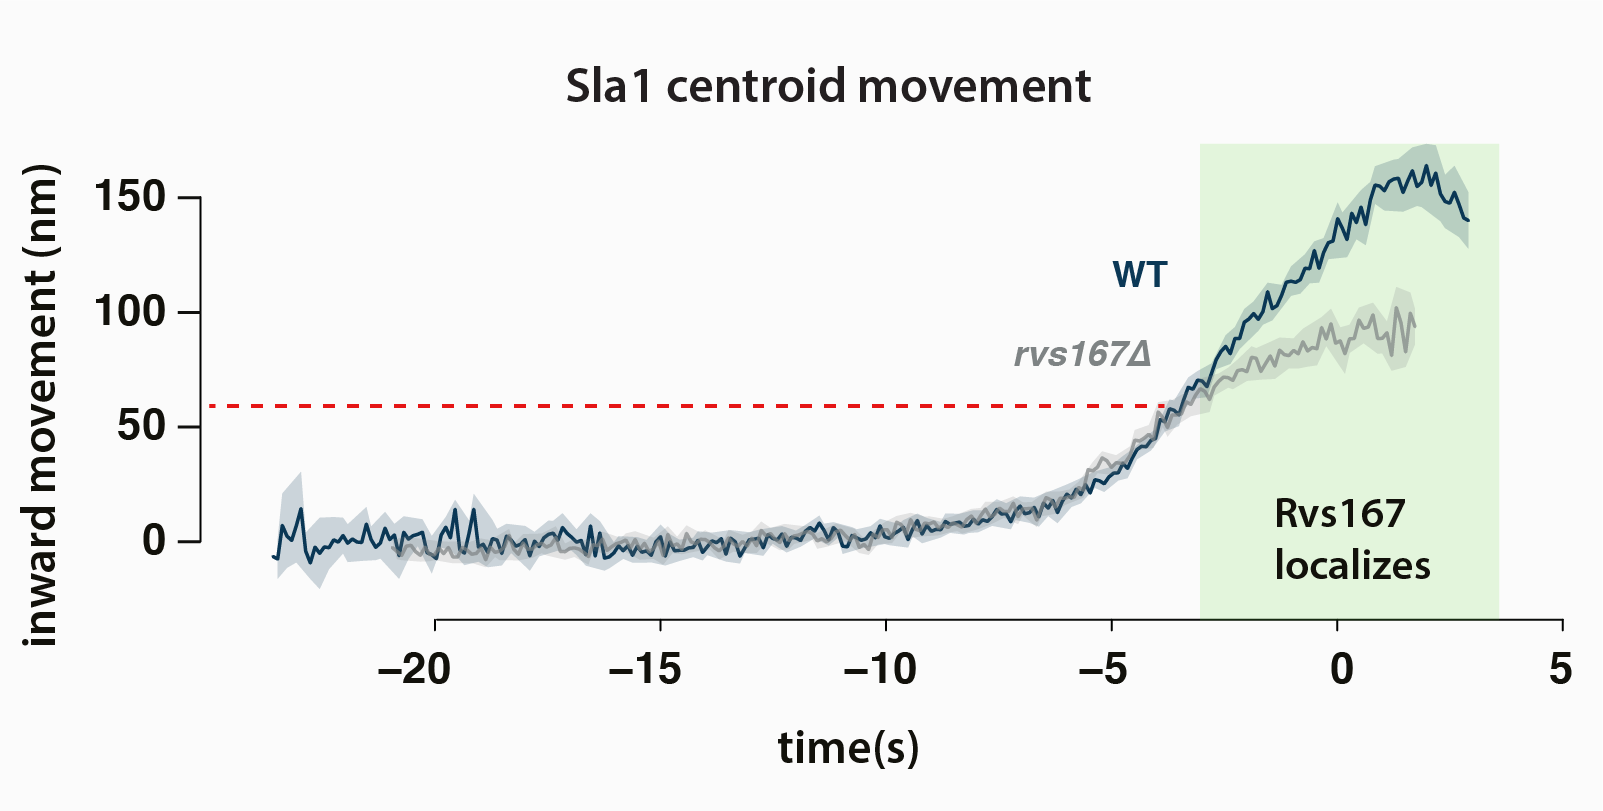
\includegraphics[width=15cm,height=20cm, keepaspectratio]{figures/results_final/rvsdeletion3}
		\caption[Coat movement in \textit{rvs167$\Delta$} cells]
		{Movement of Sla1 in WT and  \textit{rvs167$\Delta$} cells. WT Sla1 is aligned so that time=0 (sec) corresponds to scission time.Sla1 centroid  in \textit{rvs167$\Delta$} cells is shifted in time so that it moves inwards at the same time as WT Sla1. Red line indicates approximate start of deviation of \textit{rvs167$\Delta$} from WT. 
			\label{fig2_rvsdelta}
		}
	\end{figure}




\newpage
%\vspace{5mm}
CLEM has shown that Rvs167 localizes to endocytic sites after the tubes are 60nm long (Kukulski et al., 2012). Sla1 movement in \textit{rvs167$Delta$} shows therefore that membrane invagination is unaffected till Rvs is supposed to arrive. Sla1 in \textit{rvs167$Delta$} then continues to move at a much slower rate to about 80nm. That membrane scission occurs at shorter invagination lengths than in WT is corroborated by the smaller vesicles formed in \textit{rvs167$Delta$} cells (Kukulski et al., 2012).  The variability in fluorescence intensity also increases, similar to in WT Sla1 after scission. In WT cells, Sla1 continues to move inward to 140nm. This indicates that first, membrane scission can occur at invagination lengths of 80nm. Then, that the arrival of Rvs prevents membrane scission at 80nm  and allows further membrane invagination. 




%rvs167$\Delta$ 
%\textit{rvs167$\Delta$}

\section{Recruitment of Rvs and function of domains} 
\label{scaffolding_rvs}
	\paragraph{Curvature-sensing / generation by BAR proteins }
					\mbox{}\\
Cellular membrane shape is a result of properties like membrane rigidity, tension, intracellular pressure, that are all influenced by lipid composition and the proteins embedded in it (Stachowiak, Brodsky and Miller, 2013; Dmitrieff and Nédélec, 2015). Since these properties oppose membrane deformation, energy is required to deform and bend it. BAR domains localize to curved membranes, but they have also been shown to generate membrane tubes and induce vesicle formation, leading to some discussion on the interplay between these functions. 


	\vspace{5mm}
			
				\subparagraph{Generating curvature }
				\mbox{}\\
BAR domains are thought to generate membrane curvature by either scaffolding the membrane or inserting an N-terminal amphipathic helix (N-helix) into the lipid bilayer. 
Scaffolding refers to interaction between the positively charged concave surface of BAR domains with negatively charged lipids. By attracting lipids to the positive surface, BAR domains are thought to induce membrane curvature. Curvature-generation by scaffolding has been proposed as a function for I-BAR, F-BAR as well as N-BAR domains (Shimada et al., 2007; Frost et al., 2008; Arkhipov, Yin and Schulten, 2009; Saarikangas et al., 2009; Pykäläinen et al., 2011). 
	\vspace{5mm}
	
N-helices similar to that of NBAR domains can generate curvature independently of the BAR scaffold mechanism (Varkey et al., 2010; Boucrot et al., 2012). Shallow insertion of the N-helix into one leaflet of a lipid bilayer causes the lipids to rearrange, and results in a difference in membrane surface area between the two leaflets (Jennifer L Gallop, 2006). This results in membrane curvature. 


	
	\vspace{5mm}
	
				\subparagraph{Sensing curvature }
								\mbox{}\\
BAR domains show preferential binding to membranes that correlate to their intrinsic curvature: flat F-BAR domain proteins are found at flat membranes, N-BAR domains are found at tubular structures (Henne et al., 2010; Picco et al., 2015). That BAR domains are able to generate curvature does not imply that this is their function. \textit{In vivo}, the significance of curvature-generation is not determined. Tracking over thirty different endocytic proteins in mouse fibroblasts by TIRF imaging showed that Endophilin and Amphiphysin arrive late in the endocytic timeline right before scission (Taylor, Perrais and Merrifield, 2011), suggesting they arrive when membrane tubes are already formed. 


	\vspace{5mm}
Curvature-generation and sensing are likely intrinsically coupled mechanisms. BAR proteins that can induce curvature could also sense curvature: there could be feedback between curvature-sensing and generation. In the case of Rvs, the complex localizes to sites once membrane curvature is established. Whether this localization is dependent on membrane curvature, recognized by the BAR domain is not known. 


\newpage

	\subsection{BAR domains sense membrane curvature}
\label{sub_curvature}
	\vspace{2mm}
\underline{BAR domains are recruited to endocytic sites}
To test whether Rvs is recruited because of membrane curvature, I looked at the recruitment of Rvs167 without the SH3 domain, that is only the BAR domain. Cells that contain only the Rvs167 BAR domain are referred to as BAR cells. I use BAR-GFP to test first whether Rvs167 can localize without the SH3 domain, and then if it does, whether the localization is dependent on membrane curvature.

	\vspace{5mm}
BAR-GFP forms cortical patches (Fig.3.2A) in cells with curvature, so the BAR domain alone is able to localize to the plasma membrane. In yeast cells expressing both BAR-GFP and Abp1-mCherry, BAR-GFP co-localizes with Abp1-mCherry, indicating that BAR domains are recruited to endocytic patches  (Fig.\ref{fig2_sla2del}A, C).  



	\vspace{5mm}
	\underline{BAR domains sense membrane curvature \textit{in vivo}}
In order to test the curvature dependence of this localization, I compared the dynamics of Rvs167-GFP against BAR-GFP in \textit{sla2$Delta$} cells (Fig.\ref{fig2_sla2del}D-F). Sla2 is a coat protein that acts as a linker between the membrane and actin cytoskeleton. It binds membrane via its N-terminal ANTH domain and actin by the C-terminal THATCH domain. This allows forces generated by the actin network to be transmitted to the membrane (Skruzny et al., 2012). In \textit{sla2$Delta$} cells, rather than cortical actin patches that transiently co-localize with endocytic coat proteins, an “uncoupling phenotype” is observed (Kaksonen, Sun and Drubin, 2003; Skruzny et al., 2012). Although endocytic coats are formed, and actin is polymerized continuously at these sites, the membrane is not pulled inward, and vesicles are not formed. Forces generated by the actin network are not transmitted to the membrane (Fig.\ref{fig2_sla2del}E) and the membrane is not curved. If the BAR localized to endocytic sites by sensing curvature, BAR-GFP would not form cortical patches in textit{sla2$Delta$} cells.

	\vspace{5mm}

Full-length Rvs167 is recruited to the plasma membrane in \textit{sla2$Delta$} cells  (Fig.\ref{fig2_sla2del}D,F, along with Abp1. Some Rvs167 patches persist at the plasma membrane, while many are assembled and disassembled. In \textit{sla2$Delta$} cells expressing BAR-GFP, localization is removed except for rare transient patches at the plasma membrane. This shows that the BAR domain requires membrane curvature to localize. Full-length Rvs167 is able to localize to \textit{sla2$Delta$} cells, indicating that the SH3 domain helps Rvs localization. This is discussed further in the following section. 





% \textit{sla2$\Delta$} cells \ref{fig2_sla2del} (D-F). 

 
	\begin{figure}[H]
	\centering
	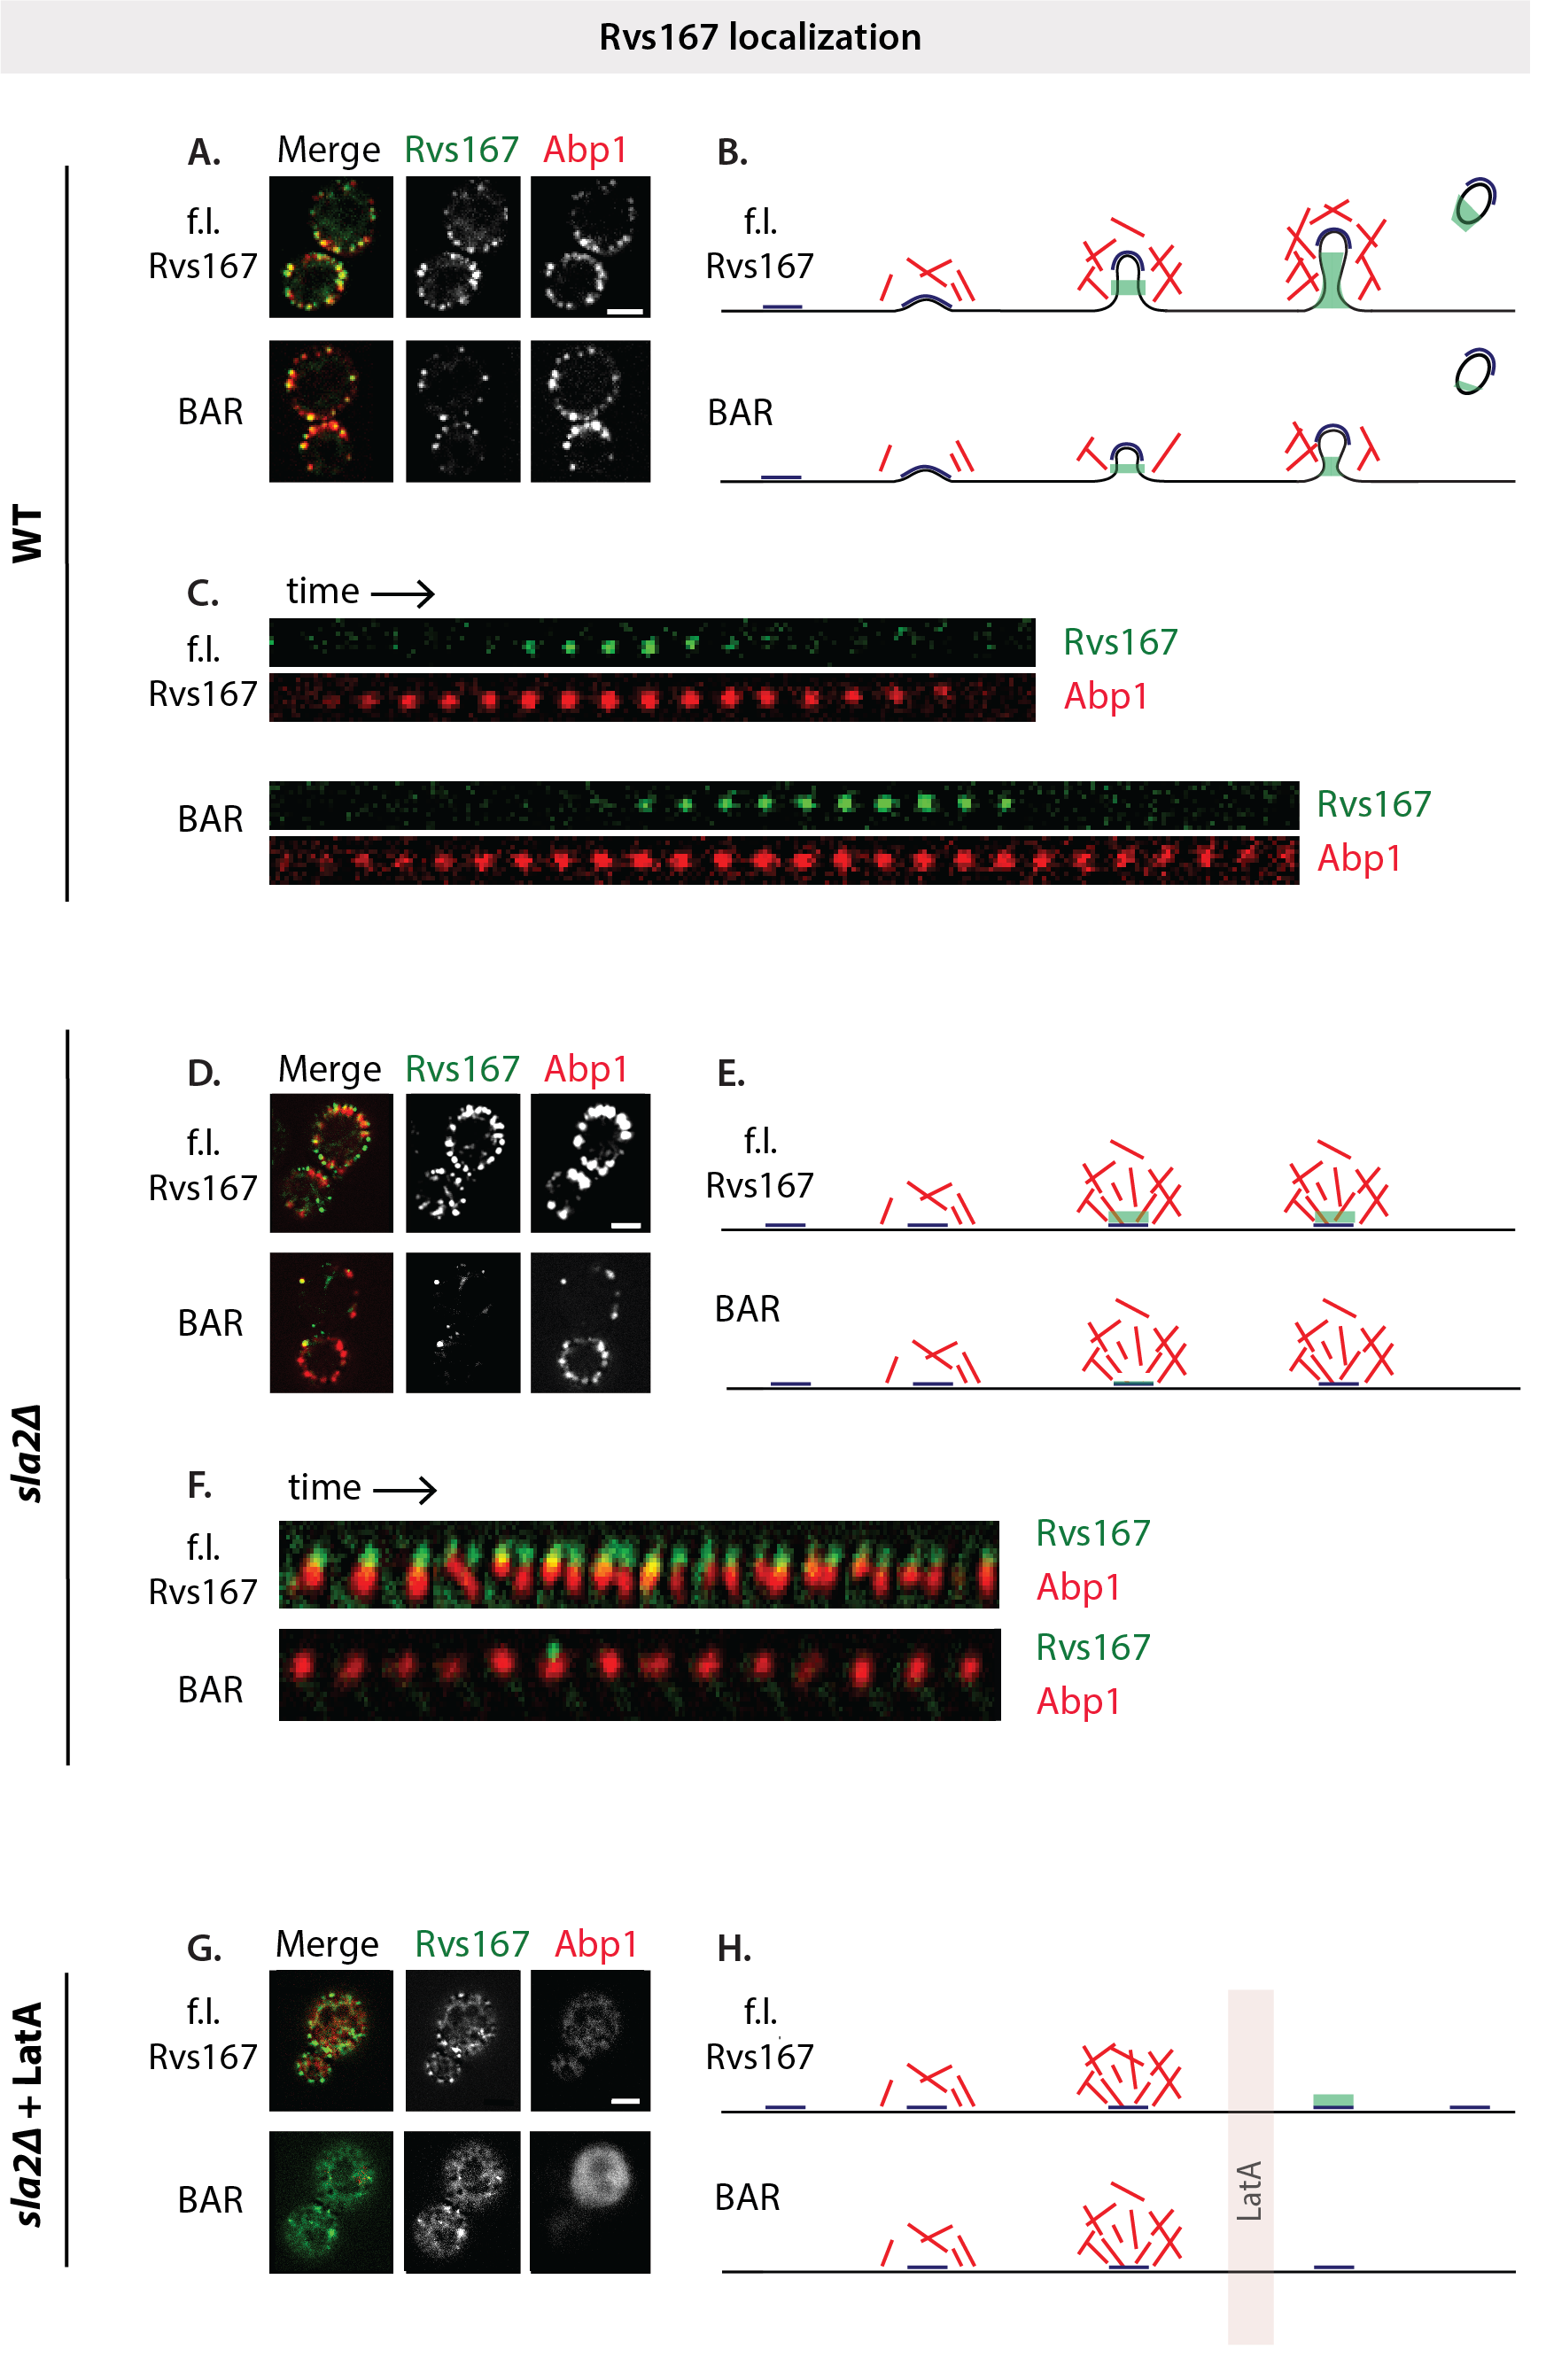
\includegraphics[width=21cm,height=21cm,keepaspectratio]{figures/results_final/sla2_del_final7}
	\caption [Localization of the Rvs167 BAR domain]
{A: Maximum intensity projection of Rvs167-GFP in WT and BAR cells, and Abp1-mCherry. Exposure 250ms. B: Schematic of membrane progression in WT and BAR  (see section \ref{delsh3_movement}).
C: Montage of Rvs167-GFP in WT and BAR cells, and Abp1-mCherry. Time between frames= 750ms.
D: Max. int.projection of Rvs167-GFP and Abp1-mCherry in \textit{sla2$\Delta$} and \textit{sla2$\Delta$}BAR cells, 
E: Schematic of membrane invagination in  \textit{sla2$\Delta$}. F: Montage of Rvs167-GFP and Abp1-mCherry in WT and BAR cells. Exposure 1000ms for GFP, 800ms for RFP. 
G: Max. int. projection of Rvs167-GFP and Abp1-mCherry in \textit{sla2$\Delta$} and \textit{sla2$\Delta$}BAR cells after treatment with LatA for 10’. Exposure 1000ms for GFP, 800ms for RFP. H: Schematic of membrane invagination in \textit{sla2$\Delta$} cells treated with LatA. 
All scale bars = 2um.
	\label{fig2_sla2del}}
	\end{figure}



	\subsection{The SH3 domain is able to localize Rvs in an actin and curvature-independent manner}
	\label{delsh3_latA}
As I show in \ref{sub_curvature}, full-length Rvs167 is able to localize to endocytic patches in \textit{sla2$\Delta$} cells. This localization must be dependent on the SH3 domain, since the BAR domain alone does not localize in \textit{sla2$Delta$} cells. SH3 domains of Rvs167 are known to interact with many actin associated proteins: an interaction with Abp1 has been shown, as well as with Las17, type I myosins, and Vrp1. 

	\vspace{5mm}
	
In order to test whether it interacts with an actin binding protein, I imaged BAR-GFP and full-length Rvs167-GFP in \textit{sla2$\Delta$} cells treated with the actin sequestering agent LatrunculinA (LatA). LatA is a sea-sponge toxin that binds monomeric actin and prevents incorporation of actin into filaments. Since high actin turnover is required at endocytic sites, LatA effectively disassembles the actin network, and blocks endocytosis. In \textit{sla2$\Delta$} cells treated with LatA, membrane curvature as well as actin and actin-binding proteins are removed from endocytic sites. Removal of the actin network after LatA is confirmed by imaging Abp1 after treatment.

	\vspace{5mm}
Surprisingly, full-length Rvs167 is transiently localized to the plasma membrane in \textit{sla2$\Delta$} cells treated with LatA (Fig.\ref{fig2_sla2del}G, H). This localization does not depend on BAR-membrane interaction, since BAR-GFP patches are not seen in similarly treated cells. This suggests that the SH3 domain is able to recruit Rvs to the plasma membrane in the absence of curvature and actin network components. Rvs167-GFP patches are transient, so assembly and disassembly of an Rvs patch can be mediated by the SH3 domain. Localization of Rvs161, which does not have an SH3 domain, is removed by LatA treatment in WT cells (Kaksonen, Sun and Drubin, 2003), supporting the conclusion that the SH3 domain drives the localization of full-length Rvs167 in \textit{sla2$\Delta$}  cells, as well as in \textit{sla2$\Delta$} cells with LatA. 


	\subsection{Loss of the SH3 domain affects progression of \\endocytic sites}
	\label{delsh3_movement}
The BAR domain was expected to act as the functional module of the Rvs complex: phenotypes of \textit{rvs167$\Delta$}  such as non-viability on starvation, and mis-localization of actin can be effectively rescued by expression of the BAR domain alone (Sivadon, Crouzet and Aigle, 1997). Since the SH3 domain unexpectedly influences localization of Rvs, I investigated its effect further.

	\vspace{5mm}
The SH3 domain generally mediates protein-protein interaction by binding to proline-rich sequences that contain a core PXXP motif (Mayer, 2001; Verschueren et al., 2015) (where X is any amino acid). These domains are ubiquitous in cellular interaction pathways, and several endocytic proteins have at least one SH3 domain. Although SH3 domains are abundant, they appear to have specific binding partners. For Rvs167, neither binding partner, nor function of the SH3 domain is clear. 


	\vspace{5mm}
\underline{Rvs recruitment and inward movement is reduced}

In order to probe the contribution of the Rvs SH3 domain to endocytosis, I studied Sla1 and BAR-GFP in BAR cells, and quantified the number of molecules recruited to endocytic sites as in Picco et al.,(Picco et al., 2015). Fig.\ref{fig2_sh3del}C shows that recruitment of BAR is reduced to half that of Rvs167 (57 +/- 9.9 for BAR compared to 113.5 +/- 5.3 for Rvs167). Cytoplasmic concentration of Rvs167 and BAR are not different (see \ref{Ch:Methods}). This indicates that although the BAR is expressed at the same level at WT Rvs167, it is recruited less efficiently. 
The inward jump of BAR is less that that of full-length Rvs167 (Fig.\ref{fig2_sh3del}A). The decrease in inward jump indicates that the position of the newly formed vesicle in BAR cells is lower than in WT. This would imply that the coat movement is reduced in BAR cells compared to WT.

\newpage
	\underline{Coat movement and actin recruitment is reduced}
	
Movement of the coat protein Sla1 is similarly reduced (Fig.\ref{fig2_sh3del}A). Sla1 moves into the cytoplasm approximately 60nm instead of the 140nm found in WT invaginations. Tubular invaginations are formed in BAR cells, and qualitatively resemble that in WT cells, as seen by CLEM  (Fig.\ref{fig2_sh3del}E). Invagination lengths in BAR cells measured by CLEM averages 35 nm +/- 13 (mean +/- standard deviation), compared to 107.6 +/- 30. Short invaginations with a maximum of 60nm have been observed in  \textit{rvs167$\Delta$} cells  by CLEM(Kukulski et al., 2012), which is about the same length as those observed in the SH3 deletion. 
Abp1 recruitment in BAR cells is reduced to 50\% of WT recruitment, to 172.6 +/- 12.9 from 347+/- 30.6 molecules in WT (Fig.\ref{fig2_sh3del}C). This data shows that loss of the SH3 domain is detrimental to the function of the Rvs complex. 


	\vspace{5mm}
		\underline{Rvs recruitment in BAR cells is delayed}
		
To check if there was a change in the timing of endocytic progression, I quantified the lifetimes of BAR, Sla1 and Abp1 in BAR cells using total internal reflection fluorescence (TIRF) microscopy. Unlike epifluorescence microscopy at the equatorial plane, in TIRF only fluorophores up to a depth of about 100nm from the glass-sample interphase are excited. This reduces fluorescent signal from the cytoplasm, allowing detection of low intensity fluorescent signal, and is a better method for quantification of protein lifetime than epifluorescence microscopy. Although this method is sensitive to low fluorescent intensity, as the proteins start to move inward into the cytoplasm, fluorescent intensity rapidly drops, because of the limited excitation depth. Therefore, rather than a quantification of the entire lifetime of the protein, this is a quantification of the non-motile lifetime of a protein that arrives at endocytic sites. Non-motile lifetimes of Rvs167, Sla1 and Abp1 are thus compared between BAR and WT cells. 

\newpage
While lifetimes of Rvs167 and Sla1 are similar in both cell types, there is a significant increase in the lifetime of Abp1 in BAR cells (Appendix). Comparable increase in lifetime of Abp1 is also seen by epifluorescence microscopy (Fig.\ref{fig2_sh3del}B). I then looked for differences in the sequence of recruitment of these proteins by looking at the difference in time between recruitment of Sla1 and Rvs167, and the difference in time between recruitment of Abp1 and Rvs167. The time difference between recruitment of Sla1 and Rvs167 is unchanged between WT and BAR cells, while the difference in time between recruitment of Abp1 and Rvs167 is increased in BAR cells  (Fig.\ref{fig2_sh3del}D).

	\vspace{5mm}
Taken together these data suggest that the BAR domain alone cannot reproduce the function of the Rvs167 at endocytic sites: recruitment of Rvs, coat and actin dynamics are all affected by the absence of the SH3 domain. 


\begin{figure}[H]
	\centering
	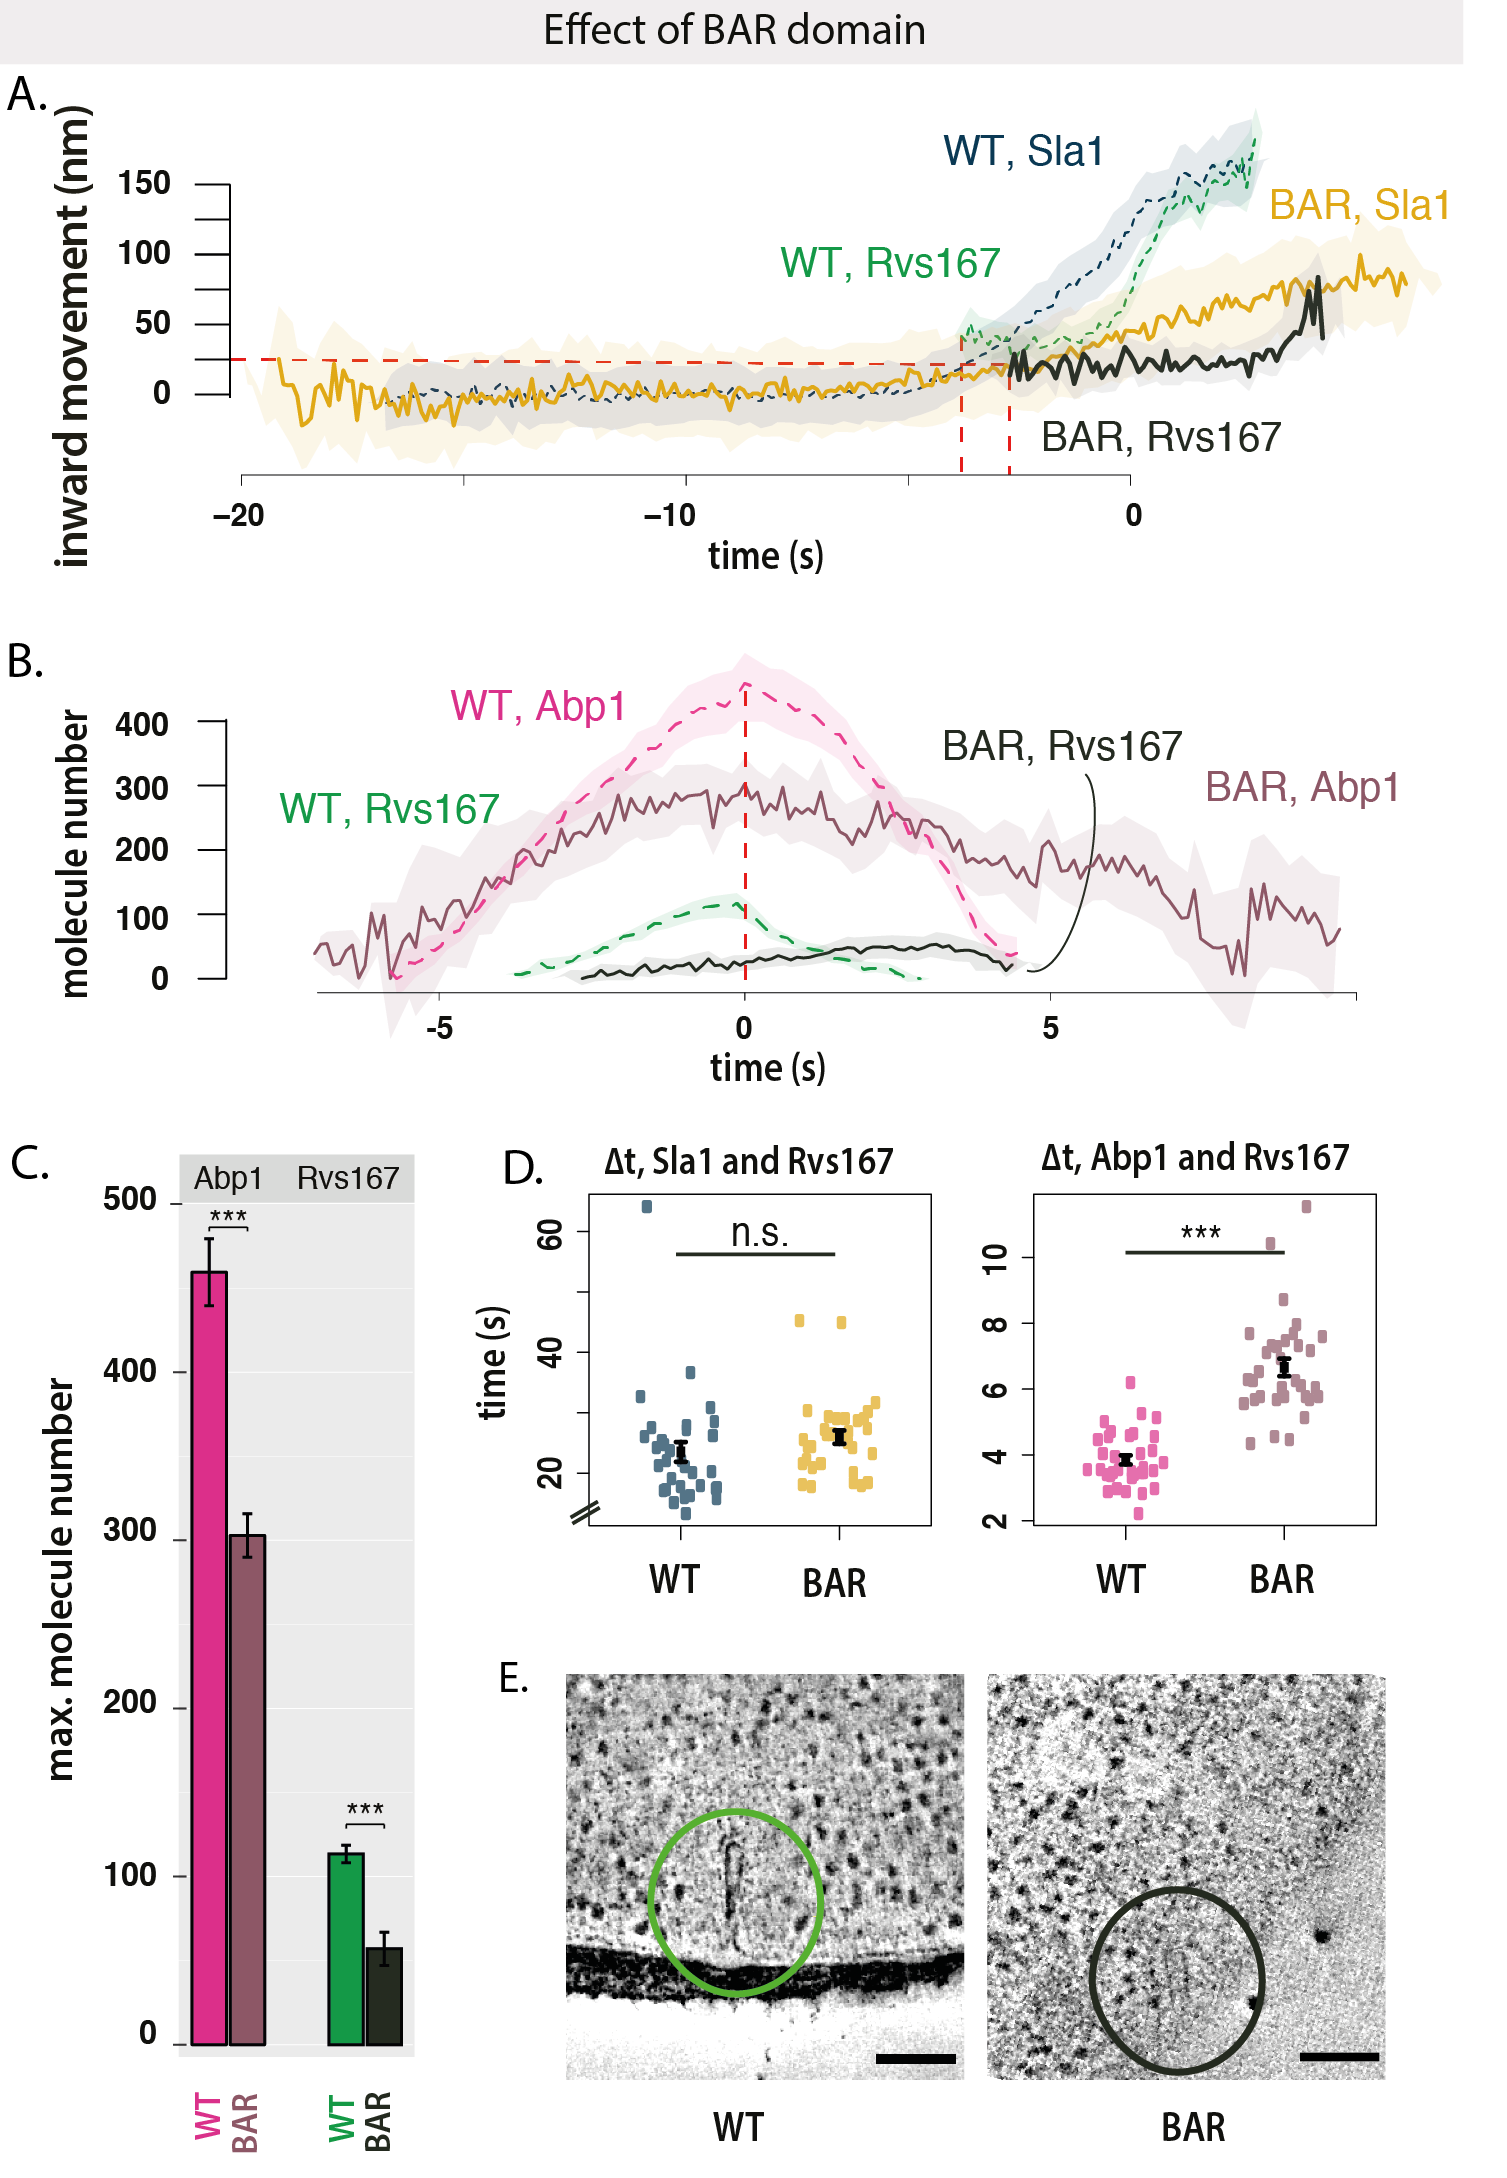
\includegraphics[width=21cm,height=21cm,keepaspectratio]{figures/results_final/delsh3_8}
	\caption [Tracking endocytic proteins in BAR cells]
	{A: Movement of Sla1 and Rvs167 in WT and BAR strains. All centroid movements are aligned so that time=0 (s) corresponds to scission time. 
	C: Molecule numbers of Abp1-GFP and Rvs167-GFP in WT and BAR cells. P-values from two-sided z test, * = p $\leq$ 0.05 , ** = p$\leq$ 0.01, *** = p $\leq$ 0.001. 
	D: Time difference between arrival of Sla1 or Abp1 and Rvs167  in WT and BAR cells. Time difference measured from TIRF images of  Rvs167-GFP/ Abp1-mCherry and Rvs167-GFP/ Sla1-mCherry. Mean and standard error of the mean are shown. p values of two-sided t test,  * = p$\leq$ 0.05, ** = p$\leq$ 0.01, *** = p$\leq$ 0.001. 
	E: Z-stack of slices from reconstructed tomograms of WT and BAR strains expressing Rvs167-GFP and Abp1-mCherry.  Scale bar=100nm.
	\label{fig2_sh3del}}

	\end{figure}
	\vspace{5mm}
	
		
\section{Function of Rvs}

%	\subsection{BAR domains as scaffold for dynamin}

%		\mbox{}\\
%While work on membrane scission in mammalian cells has converged on the idea that it is caused by dynamin interaction with BAR domains, in yeast what causes the final shape-transition from tubes to vesicles is not determined. 
While work in mammalian cells has converged on the idea that membrane scission is caused by dynamin acting in concert with BAR domain proteins, in yeast what causes the final shape-transition from tubes to vesicles is not determined. Several scission mechanisms for yeast endocytosis have been proposed in the last years, in the absence of conclusive mechanistic evidence. We know that Rvs plays a major role in determining the efficiency of membrane scission, and that in its absence membrane invaginations are shorter than in WT. I have therefore focused of models of membrane scission that assign a central role to BAR domain proteins. In the following pages, I discuss their propositions, describe experiments that have tested these mechanisms, and the conclusions they propose. 


\vspace{3mm}
\subsection{Hypothesis: Rvs is an interaction surface for membrane constriction by dynamin }
	\mbox{}\\
Yeast dynamin is the obvious solution to membrane scission. None of the three dynamin-like yeast proteins has a proline-rich domain that typically bind BAR domains, but one of them- Vps1 has been suggested to function like the mammalian dynamin in endocytic scission (Nannapaneni et al., 2010; Rooij et al., 2010). Rooij et al.,2010 propose that Vps1 localizes to endocytic sites at scission stage, and report that in \textit{vps1$\Delta$}\textit{rvs167$\Delta$} cells, rates of coat retraction after invagination increases. Coat retraction after invagination is an indication of membrane scission failure (Kaksonen, Toret and Drubin, 2005). Vps1-GFP does not localize to endocytic sites in Gadila et at.,(Goud Gadila et al., 2017), but localizes to the golgi body and to vacuoles. Kishimoto et al(Kishimoto et al., 2011), do not find a co-localization between Vps1 and Abp1, and find that the \textit{vps1$\Delta$}\textit{rvs167$\Delta$} cells do not show increased coat retraction rates. Vps1 tagged with GFP as well as superfolder GFP, and imaged by TIRF microscopy fails to co-localize with Abp1 (data from Andrea Picco, not shown). The debate concerning the involvement of Vps1 in membrane scission has been compounded by the possibility that the GFP tag on Vps1 could interfere with its localization to endocytic sites, and/or its interaction with the Rvs complex. If Vps1 is required for membrane scission, Sla1 would undergo delayed or failed scission in its absence, and Rvs dynamics would be affected. 



			\subsubsection{Vps1 does not affect Sla1 or Rvs167 dynamics }
%	\vspace{5mm}
%	\textit{vps1Δ }
I investigated the role of Vps1 by studying coat and scission proteins in \textit{vps1$\Delta$} cells in order to avoid the question of whether fluorescently tagging Vps1 affects its function. 
\vspace{5mm}

\underline{\textit{vps1$\Delta$} phenotype}

\textit{vps1$\Delta$} cells exhibit a growth defect at 37C, as has been reported (Rooij et al., 2010). In \textit{vps1$\Delta$} cells, Sla1 accumulates in patches at the plasma membrane, moves inward, and disassembles like in WT. \textit{vps1$\Delta$} does not increase the rate of membrane retraction  (Fig.\ref{fig4_vpsdel1}C). 

\vspace{4mm}
	\begin{figure}[H]
	\centering
	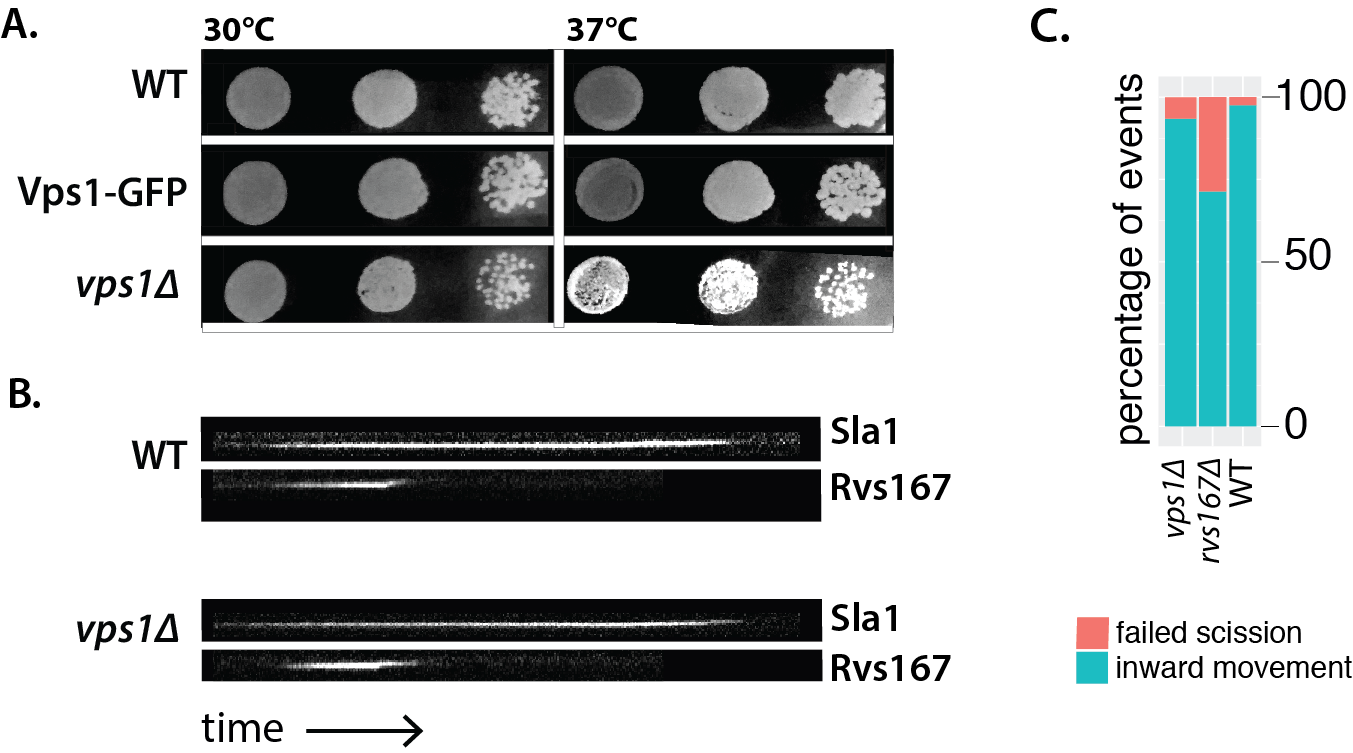
\includegraphics[width=12cm,height=12cm,keepaspectratio]{figures/results_final/vps1}
	\caption[Phenotype of \textit{vps1$\Delta$}]
	{A: Dot spots of yeast cells in WT, Vps1-GFP (diploid), and vps1Δ cell at 30C and 37C. 
		B: Kymographs of Sla1-GFP and Rvs167-GFP in WT and \textit{vps1$\Delta$} cells. Exposure 80ms.  
		C: Failure rate of membrane scission, in WT, \textit{vps1$\Delta$}, and \textit{rvs167$\Delta$}  cells. 
		\label{fig4_vpsdel1}}
\end{figure}


%\vspace{2mm}
%\ref{fig4_vpsdel2}A 

\underline{Sla1 and Rvs167 in \textit{vps1$\Delta$} cells}

Centroid movements and intensities of Sla1 and Rvs167 in time are plotted in Fig.\ref{fig4_vpsdel1}D-G. WT Sla1 is aligned so that time=0 (s) corresponds to scission time. Sla1 movement for \textit{vps1$\Delta$}   in Fig.\ref{fig4_vpsdel1}D is shifted in time so that it starts to move inward at the same time as WT. The lifetime of Sla1-GFP appears to be slightly shortened in \textit{vps1$\Delta$}   compared to the WT. However, this shortening occurs early in the lifetime of the protein at endocytic patches, when the molecule numbers of Sla1 are low, and therefore is not likely to be a directly related to the scission process. Later, similar to WT, Sla1 in \textit{vps1$\Delta$}  moves into the cytoplasm about 140nm before membrane scission occurs. Sla1 moves inward at the same rate, and to similar maxima as WT. 


\vspace{5mm}
Dynamics of Rvs167 also remains the same as in WT (Fig.\ref{fig4_vpsdel1}F,G). Magnitude of centroid movement is unchanged, indicating that the base of the vesicle formed is likely at the same position as in WT. Fluorescent intensity shows the typical sharp drop. These data indicate that Vps1 is not involved in regulating membrane scission in \textit{S. cerevisiae}.  

\vspace{5mm}

	\begin{figure}[H]
	\centering
	\includegraphics[width=14cm,height=14cm,keepaspectratio]{figures/results_final/vps2}
	\caption[Tracking endocytic proteins in \textit{vps1$\Delta$} cells]
	{A, B: Movement and normalized fluorescent intensity of Sla1 in WT and \textit{vps1$\Delta$} cells. Time =0 (s) for WT Sla1 centroid corresponds to scission time. Sla1 centroid for \textit{vps1$\Delta$} is shifted in time to begin inwards movement at the same time as WT. 
		C, D: Movement and normalized fluorescent intensity of Rvs167-GFP in WT and  \textit{vps1$\Delta$} cells. Time =0 (s) for WT Rvs167 centroid corresponds to scission time. Rvs167 for \textit{vps1$\Delta$} is shifted so that fluorescent intensity maxima is at time=0 (s).
		\label{fig4_vpsdel2}}
\end{figure}



\newpage
\subsection{Hypothesis: Rvs barrier causes line tension at lipid interphase, causing scission}
			\mbox{}\\
Phosphatidylinositols (PIs) and their lipid derivatives play important roles in many cellular processes including membrane trafficking and cell signalling. Conversion between lipid types is driven by kinases, lipases, and phosphatases and controlled throughout the membrane trafficking pathway. 


\vspace{5mm}
Phosphatidylinositol (4,5)-biphosphate (PIP\textsubscript{2}) is an important lipid type found at the cell surface, and is enriched and depleted from endocytic sites at the plasma membrane in concert with the assembly and disassembly of the endocytic machinery. Synaptojanins form a subset of inositol polyphosphate 5-phosphatases that hydrolyze PIP\textsubscript{2} to PI(4)P by removing the phosphate at the 5’ position of the inositol ring. They are known to take part in CME and intracellular signalling, as well as in modulating the actin cytoskeleton (McPherson et al., 1996). 


\vspace{5mm}
In mammalian cells, disruption of Synaptojanin genes results in cellular accumulation of PIP\textsubscript{2} at endocytic sites. Coated vesicles gather at the plasma membrane, suggesting a role for lipid hydrolysis in releasing coat proteins from nascent vesicles. Synaptojanins contain an N-terminal homology domain with the cytoplasmic domain of the yeast SAC1 gene that is implicated in lipid metabolism, actin morphology, and vesicle transport in the secretary pathway (Kearns et al., 1997). A central catalytic domain is then followed by a proline-rich C-terminal region that is the canonical interaction partner of SH3 domains. Synaptojanins interact with actin binding proteins and BAR domain proteins, potentiating also a role in membrane invagination and scission. 


\vspace{5mm}
The yeast genome encodes for three Synaptojanin-like proteins- Inp51, Inp52 and Inp53- that regulate phospholipid metabolism. In \textit{inp51$\Delta$}\textit{inp52$\Delta$}
 cells, increased lifetimes of endocytic proteins and produce aberrant membrane invaginations that could indicate scission failure and defective endocytosis (Srinivasan et al., 1997; Singer-Krüger et al., 1998). \textit{inp52$\Delta$} \textit{rvs167$\Delta$}
 cells have increase membrane retraction rates, supporting a possible role for Inp52 in membrane scission (Kishimoto et al., 2011). Loss of Inp51 leads to an increase in bulk PIP\textsubscript{2} level. Changes in PIP\textsubscript{2} levels have not been reported for mutations of Inp52, and are lipid levels not measured locally at the endocytic sites, so the effects of synaptojanin deletion to PIP\textsubscript{2} levels at endocytic sites are not established (Stolz et al., 1998; Stefan, Audhya and Emr, 2002).


\vspace{5mm}
In a model proposed by Liu et al, Synaptojanins and BAR proteins interact to regulate PIP\textsubscript{2} hydrolysis, which in turn drives membrane scission. Here, Rvs forms a scaffold on the membrane tube, and protects the underlying	PIP\textsubscript{2}  from hydrolysis. Synaptojanin arrives at inavaginated membranes, and hydrolyses unprotected	PIP\textsubscript{2}. This generates a boundary between BAR-protected 	PIP\textsubscript{2} at the tube and hydrolyzed PIP\textsubscript{2} at the bud tip. This lipid boundary produces line tension at the interphase that could generate enough force to pinch off a vesicle. 


	\subsubsection{Yeast synaptojanins do not significantly affect coat and Rvs movement } 
%\ref{fig_inp}
	
\underline{Localization and deletion phenotype of synaptojanins}

I tested the lipid hydrolysis model described above by studying the effect of synaptojanin deletion on Sla1 and Rvs167. 
Of the three yeast Synaptojanins, only Inp52-GFP localizes to cortical patches (Fig.\ref{fig_inp}D). Inp51-GFP exhibits a diffuse cytoplasmic signal, while Inp53 localizes to patches within the cytoplasm, likely to the trans-golgi network, as has been noted in other work (Bensen, Costaguta and Payne, 2000). Time alignment with other endocytic proteins, as in Picco et al., 2015 , shows that Inp52 localizes to endocytic sites at the late stage of scission, similar to Rvs. The centroid of Inp52-GFP is localized to the tip of the invaginated tube (Fig.\ref{fig_inp}D): spatial and temporal localization is consistent with influence on scission. 

%	\vspace{5mm}

		
\begin{figure}[H]
	\centering
	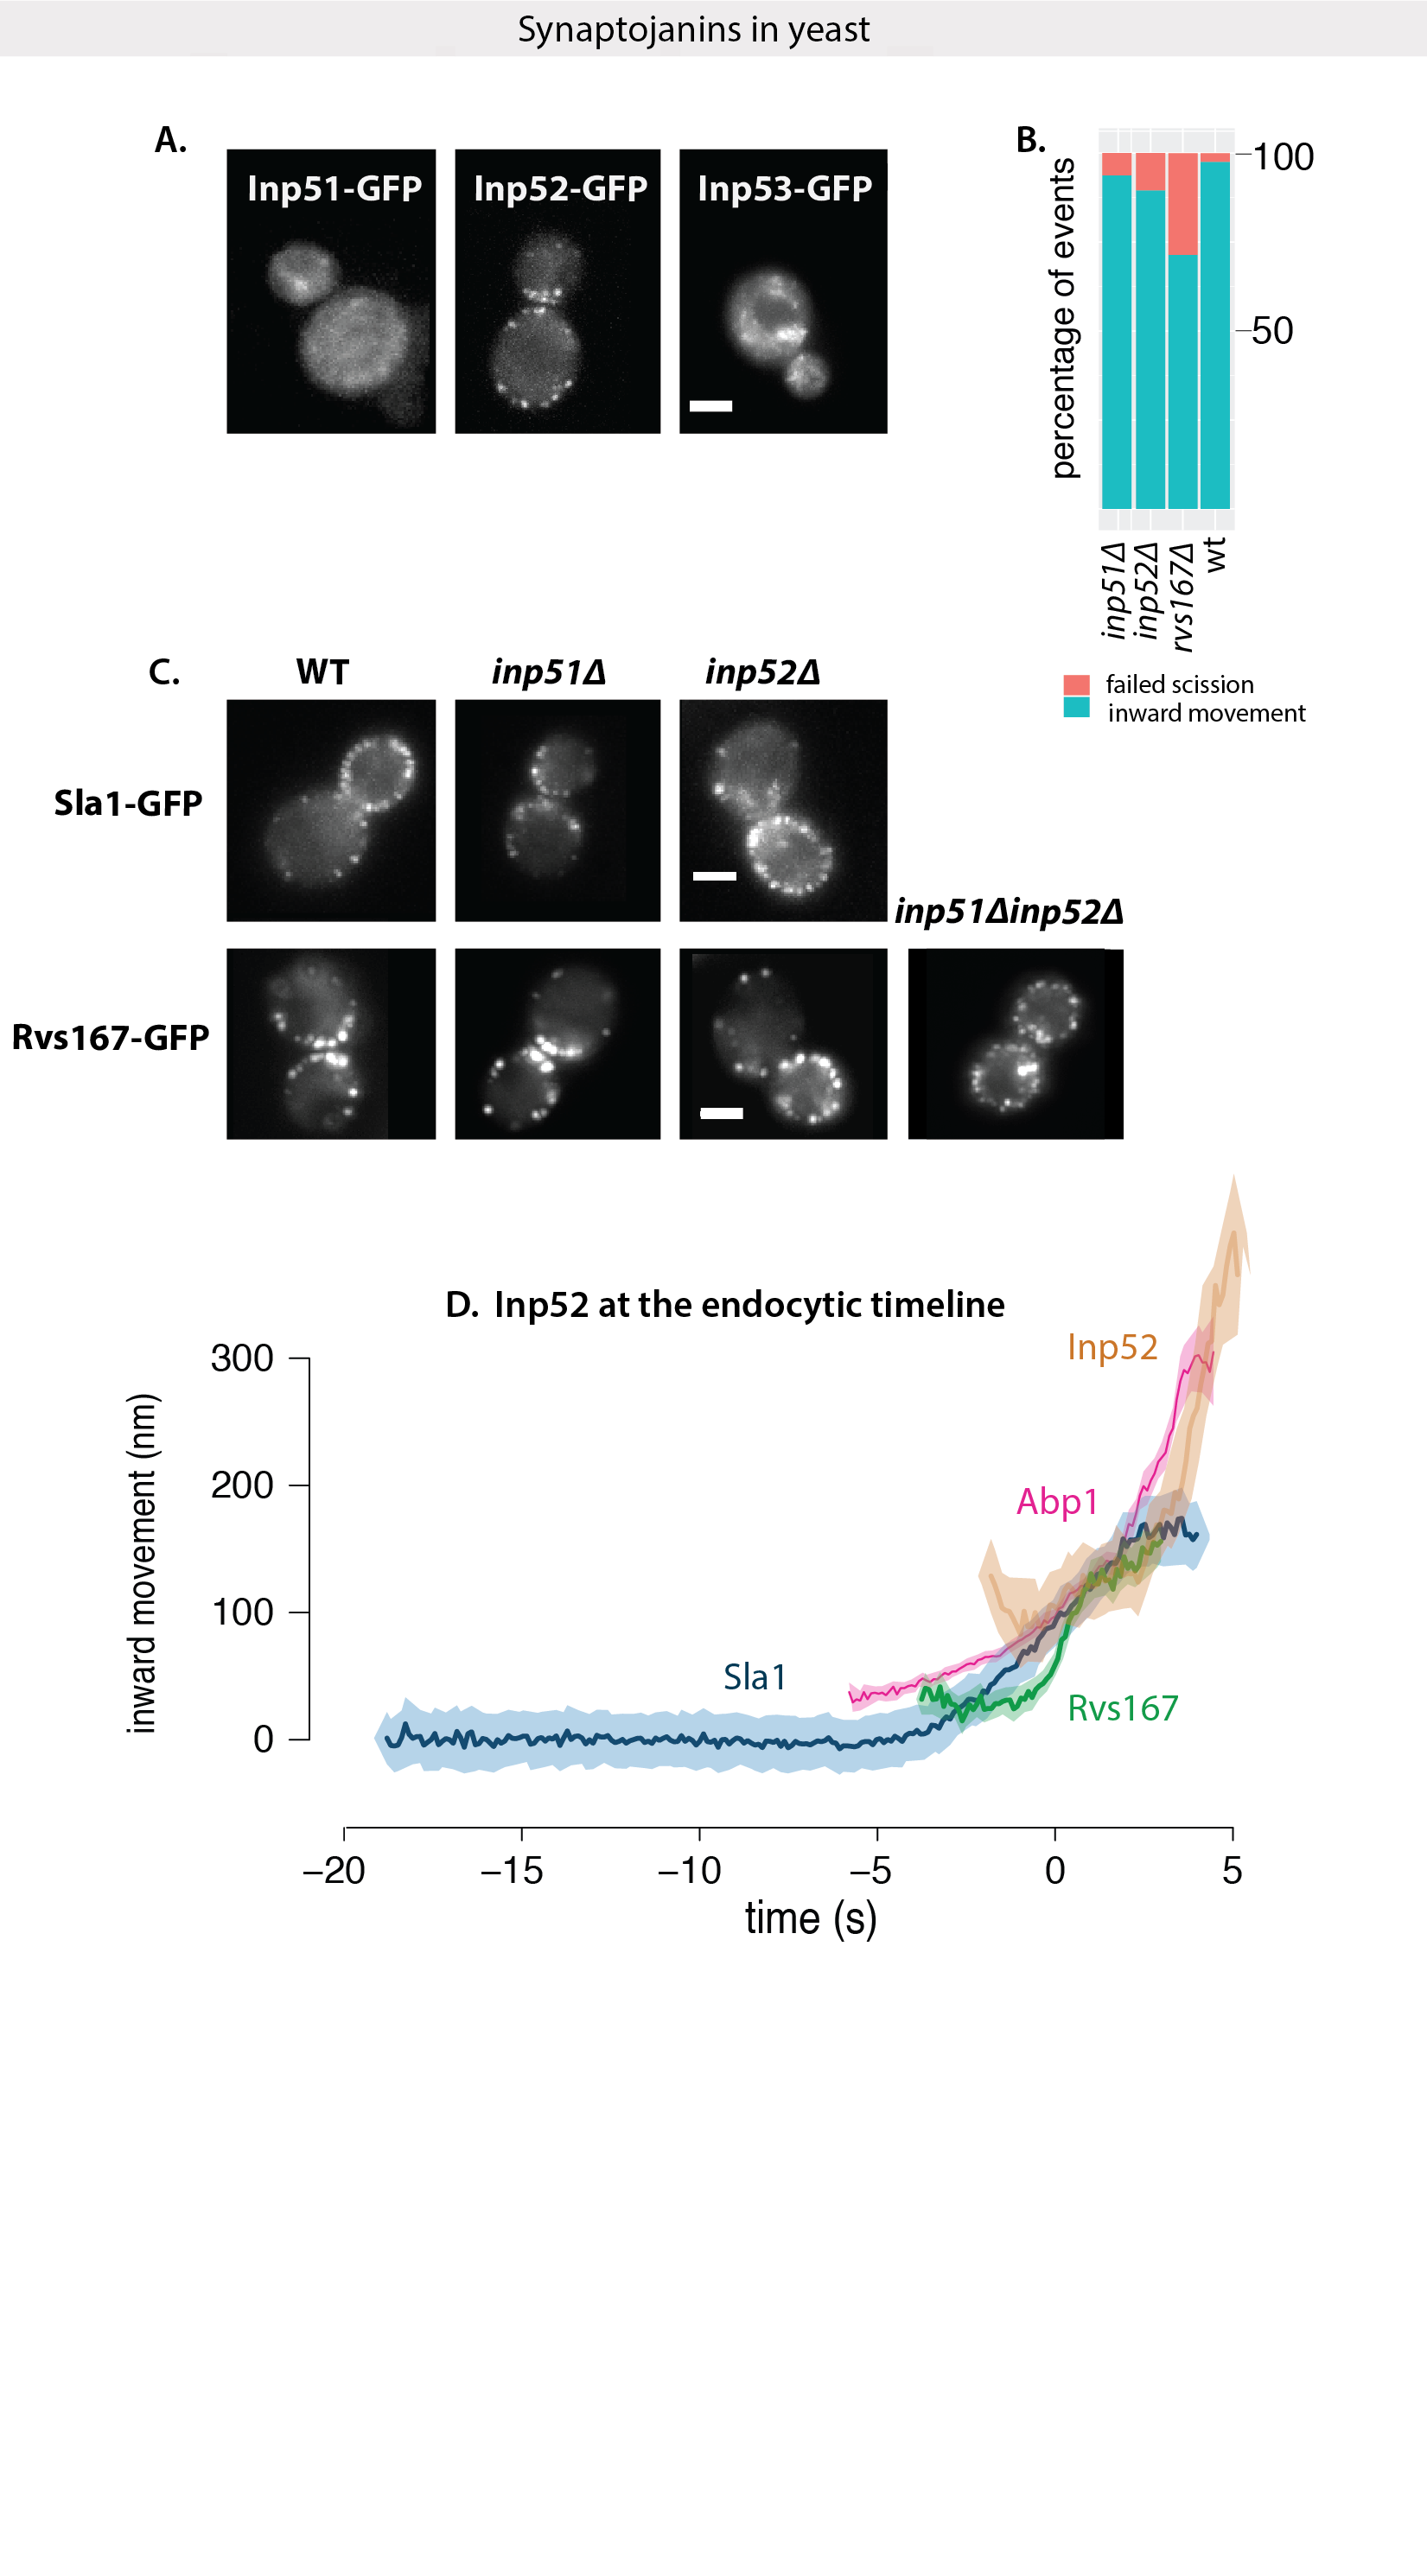
\includegraphics[width=21cm,height=21cm,keepaspectratio]{figures/results_final/inp}
	\caption[Synaptojanin-like proteins in yeast]
	{A: Maximum intensity projections of cells expressing GFP-tagged Inp51, Inp52, and Inp53. Exposure time 80ms.
		B: Failure rate of membrane scission in WT, \textit{rvs167$\Delta$}, \textit{inp51$\Delta$} and \textit{inp52$\Delta$} strains.
		C: Maximum intensity projection of Sla1-GFP in WT,  \textit{inp51$\Delta$},  \textit{inp52$\Delta$} cells. Max. int. projection of Rvs167-GFP in WT,  \textit{inp51$\Delta$},  \textit{inp52$\Delta$} and  \textit{inp51$\Delta$}\textit{inp52$\Delta$}   cells.
		D: Inp52-GFP in endocytic timeline in WT cells. Time=0 (s) is scission time.
		All scale bars =2um.
		\label{fig_inp}}
\end{figure}

	
In both \textit{inp51$\Delta$} and \textit{inp52$\Delta$} cells, Sla1-GFP patches are assembled and disassembled, as is Rvs167-GFP. Sla1 retraction rates are slightly increased to 12\% in \textit{inp52\textDelta}, compared to 2\% in WT, and 6\% in \textit{inp51$\Delta$}
(Fig.\ref{fig_inp}B). 
\vspace{5mm}

% Fig.\ref{fig_inpmov}
\underline{Sla1 and Rvs167 in synaptojanin deleted cells}

 In Fig.\ref{fig_inpmov}A, Sla1 movement in \textit{inp51$\Delta$} and \textit{inp52$\Delta$}
 cells is compared against WT. WT Sla1 is aligned in time so that time=0 (s) corresponds to scission time. Sla1 centroids for \textit{inp51$\Delta$} and \textit{inp52$\Delta$} are shifted so that they begin to move inward at the same time as WT Sla1. All three Sla1 centroids have the same rate of inward movement. While Sla1 in \textit{inp51$\Delta$} moves inward to about the same distance as WT, in \textit{inp52$\Delta$}, the centroid of Sla1 persists for nearly 5 seconds longer than WT (arrowhead in Fig.\ref{fig_inpmov}A). This centroid movement is noisier than the inward movement preceding it, and is likely from post-scission of movement of the vesicle, suggesting a delay in the disassembly of Sla1 from the vesicle. 


\vspace{5mm}	
Rvs167 dynamics are similar to WT in both \textit{inp51$\Delta$}
 and \textit{inp52$\Delta$} cells (Fig.\ref{fig_inpmov}C, D). Rvs167 centroids move inward to about the same distance into the cytoplasm as WT when they jump inward. In \textit{inp52$\Delta$} cells, however, Rvs167 patches appear to not disassemble completely (arrowhead in Fig.\ref{fig_inpmov}C) unlike in the WT. Since the fluorescent intensity begins to drop, and the delay is at the end of decay, this change in Rvs167 dynamics is likely after vesicle formation. This indicates that there is a delay in the disassembly of Rvs from vesicles in \textit{inp52$\Delta$} cells, similar to the Sla1 delay. Assembly of Rvs167 in the \textit{inp51$\Delta$}
 takes about 2 seconds longer compared to WT. The implication of this delay is not thus far clear. 

	\vspace{5mm}
The Liu et al., model predicts that if line-tension from lipid hydrolysis is removed, membrane scission should be delayed or fail. Since the differences in Sla1 and Rvs167 centroid dynamics for \textit{inp52$\Delta$} are post-scission, I find that the data is consistent with a role for Inp52 in removing Sla1 and Rvs167 from vesicles, rather than a primary role in membrane scission. 


\vspace{5mm}
I then quantified the number of Rvs167 molecules recruited to endocytic patches in \textit{inp51$\Delta$}, \textit{inp52$\Delta$}, and \textit{inp51$\Delta$} \textit{inp52$\Delta$} cells. WT levels of Rvs167 are recruited in both \textit{inp51$\Delta$} and \textit{inp52$\Delta$} cases. In \textit{inp51$\Delta$}\textit{inp52$\Delta$} cells however, nearly three times as much Rvs is recruited to sites as in WT (Fig.\ref{fig_inpmov}B). Some Rvs167-GFP patches in these cells assemble and disassemble, although the majority persist throughout the imaging time. Many large clusters of Rvs167 are present, and the regular inward jump observed in WT cells is not seen in these mutant cells. Some Rvs167 patches are also seen inside the cell far from the plasma membrane, consistent with observations of Sla1 patches deep within the cytoplasm (Sun et al., 2007). These cytoplasmic Rvs167 patches are likely formed on  aberrant membrane invaginations continuous with the plasma membrane. These membranes are able to assemble and disassemble endocytic patches (Sun et al., 2007). Some Sla1 patches are motile in \textit{inp51$\Delta$} \textit{inp52$\Delta$}, and uptake of extracellular membrane appears to proceed in spite of the morphological aberrations (Sun et al., 2007). This means that endocytic membrane scission can occur in these cells. 



\vspace{5mm}
Analysis of the \textit{inp51$\Delta$}\textit{inp52$\Delta$} phenotype is compounded by the retention of endocytic proteins on vesicles. If Rvs, coat, and other components are not recycled from vesicles, I cannot distinguish between membrane tubes and vesicles that remain in the vicinity of newly forming membrane tubes. Further, this failure to recycle proteins affects recruitment of protein to new endocytic sites and I cannot separate the effect due to failure to recruit protein from a direct effect on scission. That  the \textit{inp51$\Delta$}\textit{inp52$\Delta$} phenotypevresults in more aberrations in Rvs dynamics than single deletions suggests that the two proteins function in separate but partially overlapping pathways (Stolz et al., 1998). Defects caused by \textit{inp51$\Delta$}
are then partially compensated for by Inp52, and vice-versa, but deletion of both results in large irregularities in cellular processes.




\vspace{3mm}
		\begin{figure}[H]
	\centering
	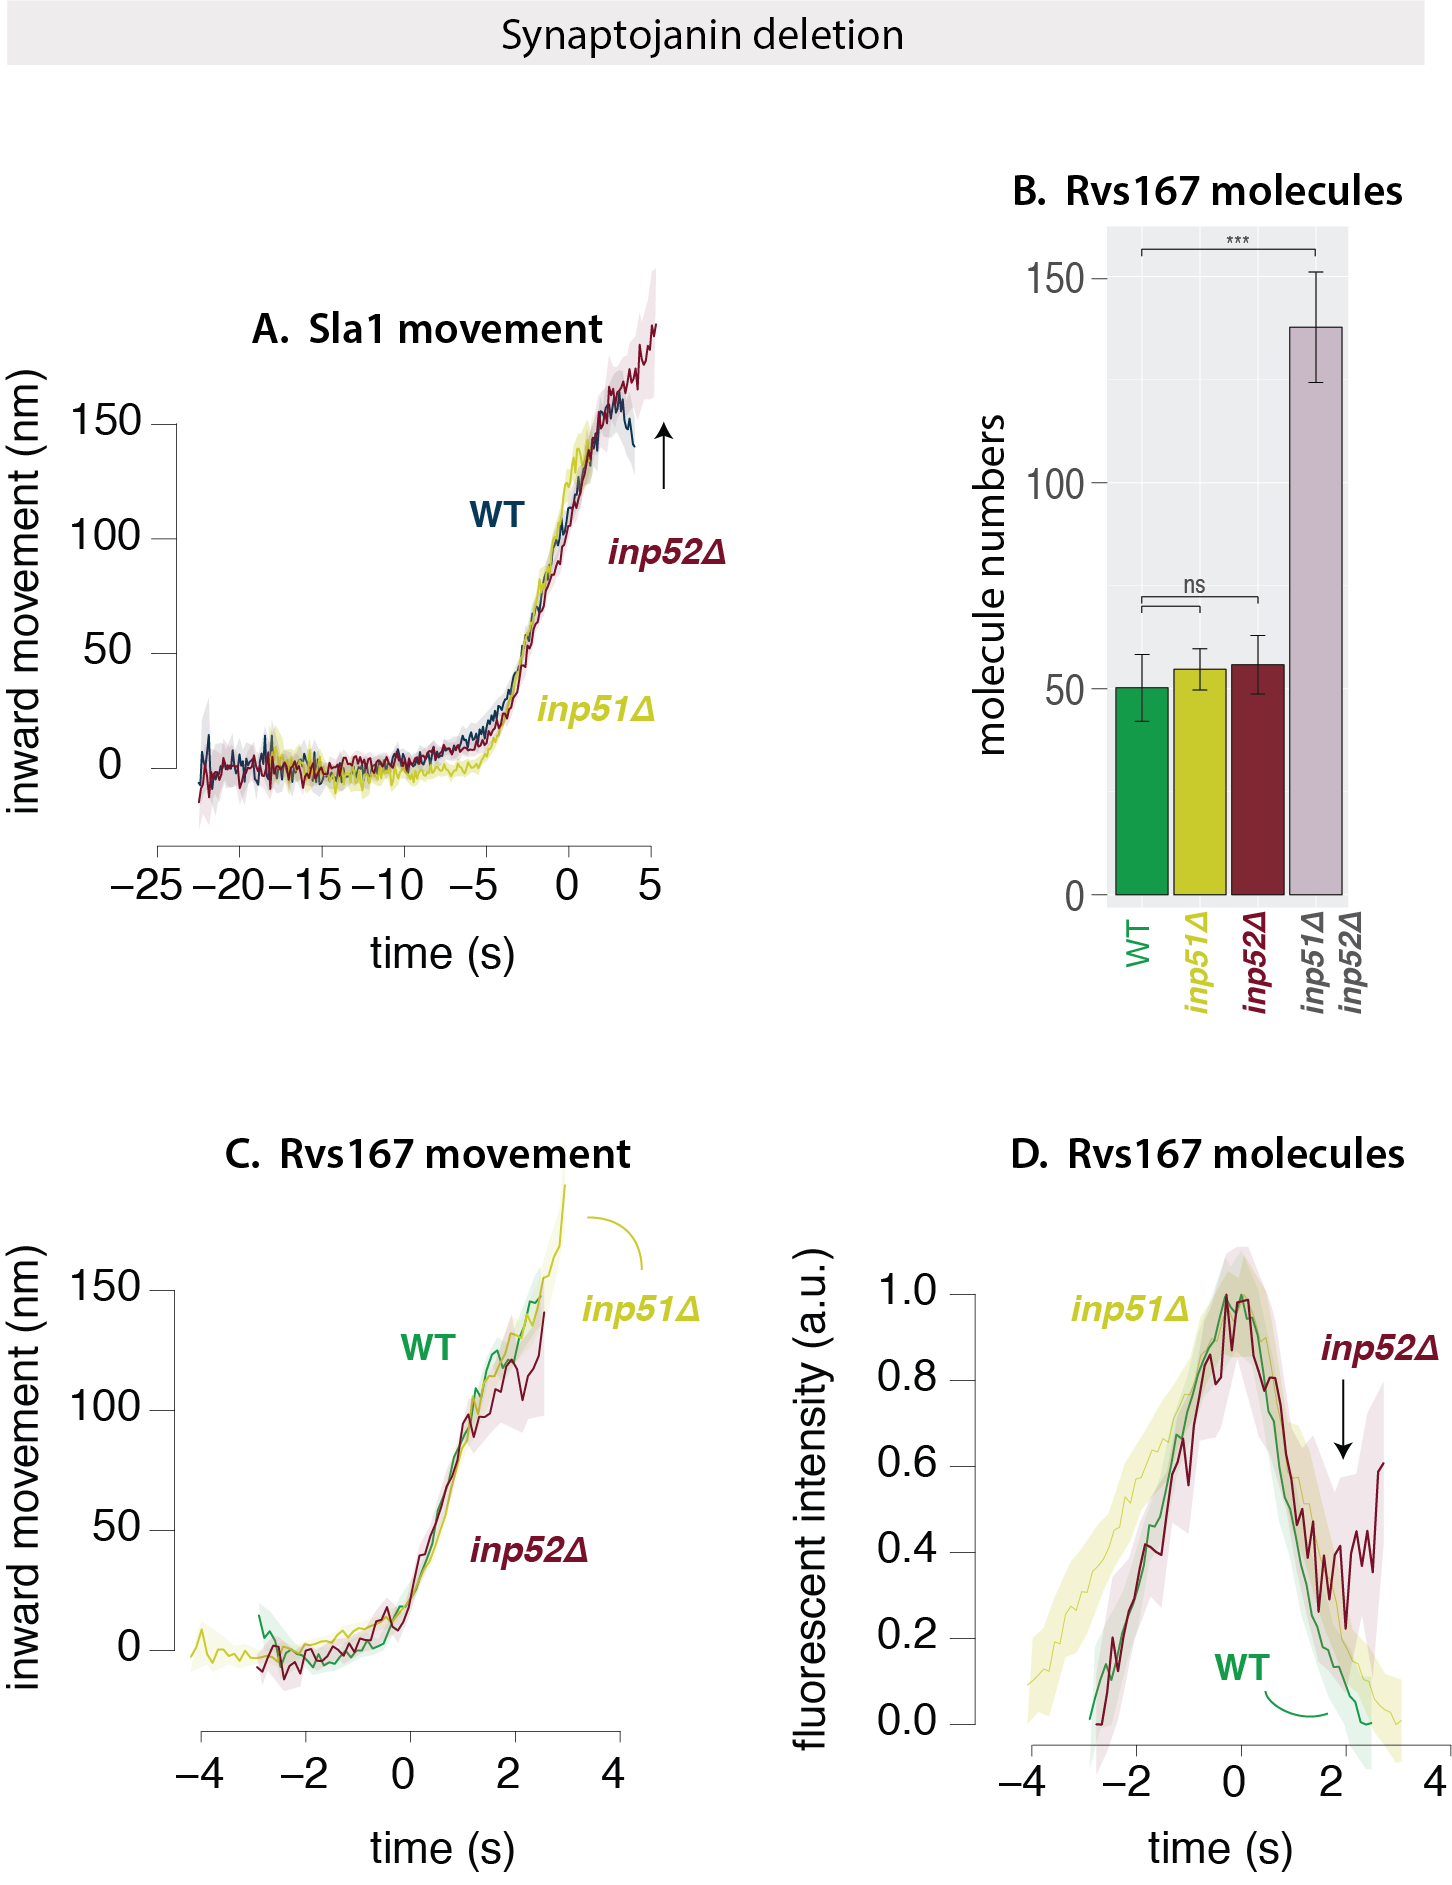
\includegraphics[width=18cm,height=18cm,keepaspectratio]{figures/results_final/inp_movement3}
	\caption[Effect of synaptojanin deletion]
{A: Movement of Sla1 in WT, \textit{inp51$\Delta$ }  and \textit{inp52$\Delta$ } cells. Time=0 (s) for WT Sla1 centroid corresponds to scission time. Sla1 centroids for \textit{inp51$\Delta$ }, \textit{inp52$\Delta$ }  are shifted to move inwards at the same time as WT. 
		B: Median number of Rvs167 molecules recruited in WT, \textit{inp52$\Delta$}, \textit{inp52$\Delta$ } and \textit{inp51$\Delta$inp52$\Delta$ } cells. P-values from two-sided z test,  * = p $\leq$ 0.05 , ** = p$\leq$ 0.01, *** = p $\leq$ 0.001.  
		C: Movement of Rvs167 in WT, \textit{inp51$\Delta$ } and \textit{inp52$\Delta$ }. 
		D: Normalized fluorescent intensity of averaged Rvs167 patches in WT, \textit{inp51$\Delta$ }, \textit{inp52$\Delta$ } cells.
		\label{fig_inpmov}}
\end{figure}


	\vspace{5mm}




\newpage

\subsection{Hypothesis: Rvs generates frictional forces on the membrane, causing scission}
				\mbox{}\\
Recent \textit{in vitro} experiments have proposed BAR-mediated protein friction as a mechanism for membrane scission (Simunovic et al., 2017). In this model, a BAR domain scaffold on a membrane tube forms a frictional barrier to lipid diffusion. Forces that pull on the membrane increase the frictional force exerted by the scaffold on the underlying membrane tube. This leads to membrane thinning in the region not covered by the BAR scaffold, since there is no lipid influx. In turn, this leads to increased membrane tension in this region. Eventually, membrane pores form in this portion of the tube and rupture the tube, forming a vesicle. \textit{In-vivo}, the forces pulling the membrane could be provided by actin polymerization.
This model predicts that if more BAR proteins are added, and at a faster rate, to the membrane, frictional force would increase. If frictional force increases, scission would occur faster: that is, at shorter invagination lengths compared to a membrane with fewer BAR proteins. 


	\subsubsection{Membrane scission is not influenced by Rvs number}
To test whether protein friction could effect membrane scission in yeast, I duplicated the Rvs161 and Rvs167 genes using a method described in Huber et al., 2014. Gene duplication was performed in haploid cells to produce strains that have two copies in tandem (2xh) of both Rvs161 and Rvs167 genes. Thes haploid strains were then mated to generate diploid strains that have four copies of Rvs161 and Rvs167 genes (4xd). WT diploid strains have two copies of Rvs genes (WT in diploids: 2xd). Cells containing 1x copy of Rvs161 and Rvs167 (1xd) were generated by crossing an \textit{rvs167$\Delta$}
 strain with an \textit{rvs161$\Delta$} strain. The diploid strains allow comparison of effects within a wider range of Rvs gene copy number. 



	



%In Fig.\ref{fig_rvshaploid}A, Sla1 movement in WT (1xh) and Rvs duplicated (2xh) haploids are presented. WT Sla1 is aligned so that time= 0 (s) corresponds to scission time. Sla1 for 2xh is shifted so that it moves inwards at the same time as WT. Both Sla1 centroids move inwards at the same rate, and to the same distance of 140nm, indicating that membrane invagination is not affected by adding more copies of the Rvs genes. 

				\begin{figure}[H]
	\centering
	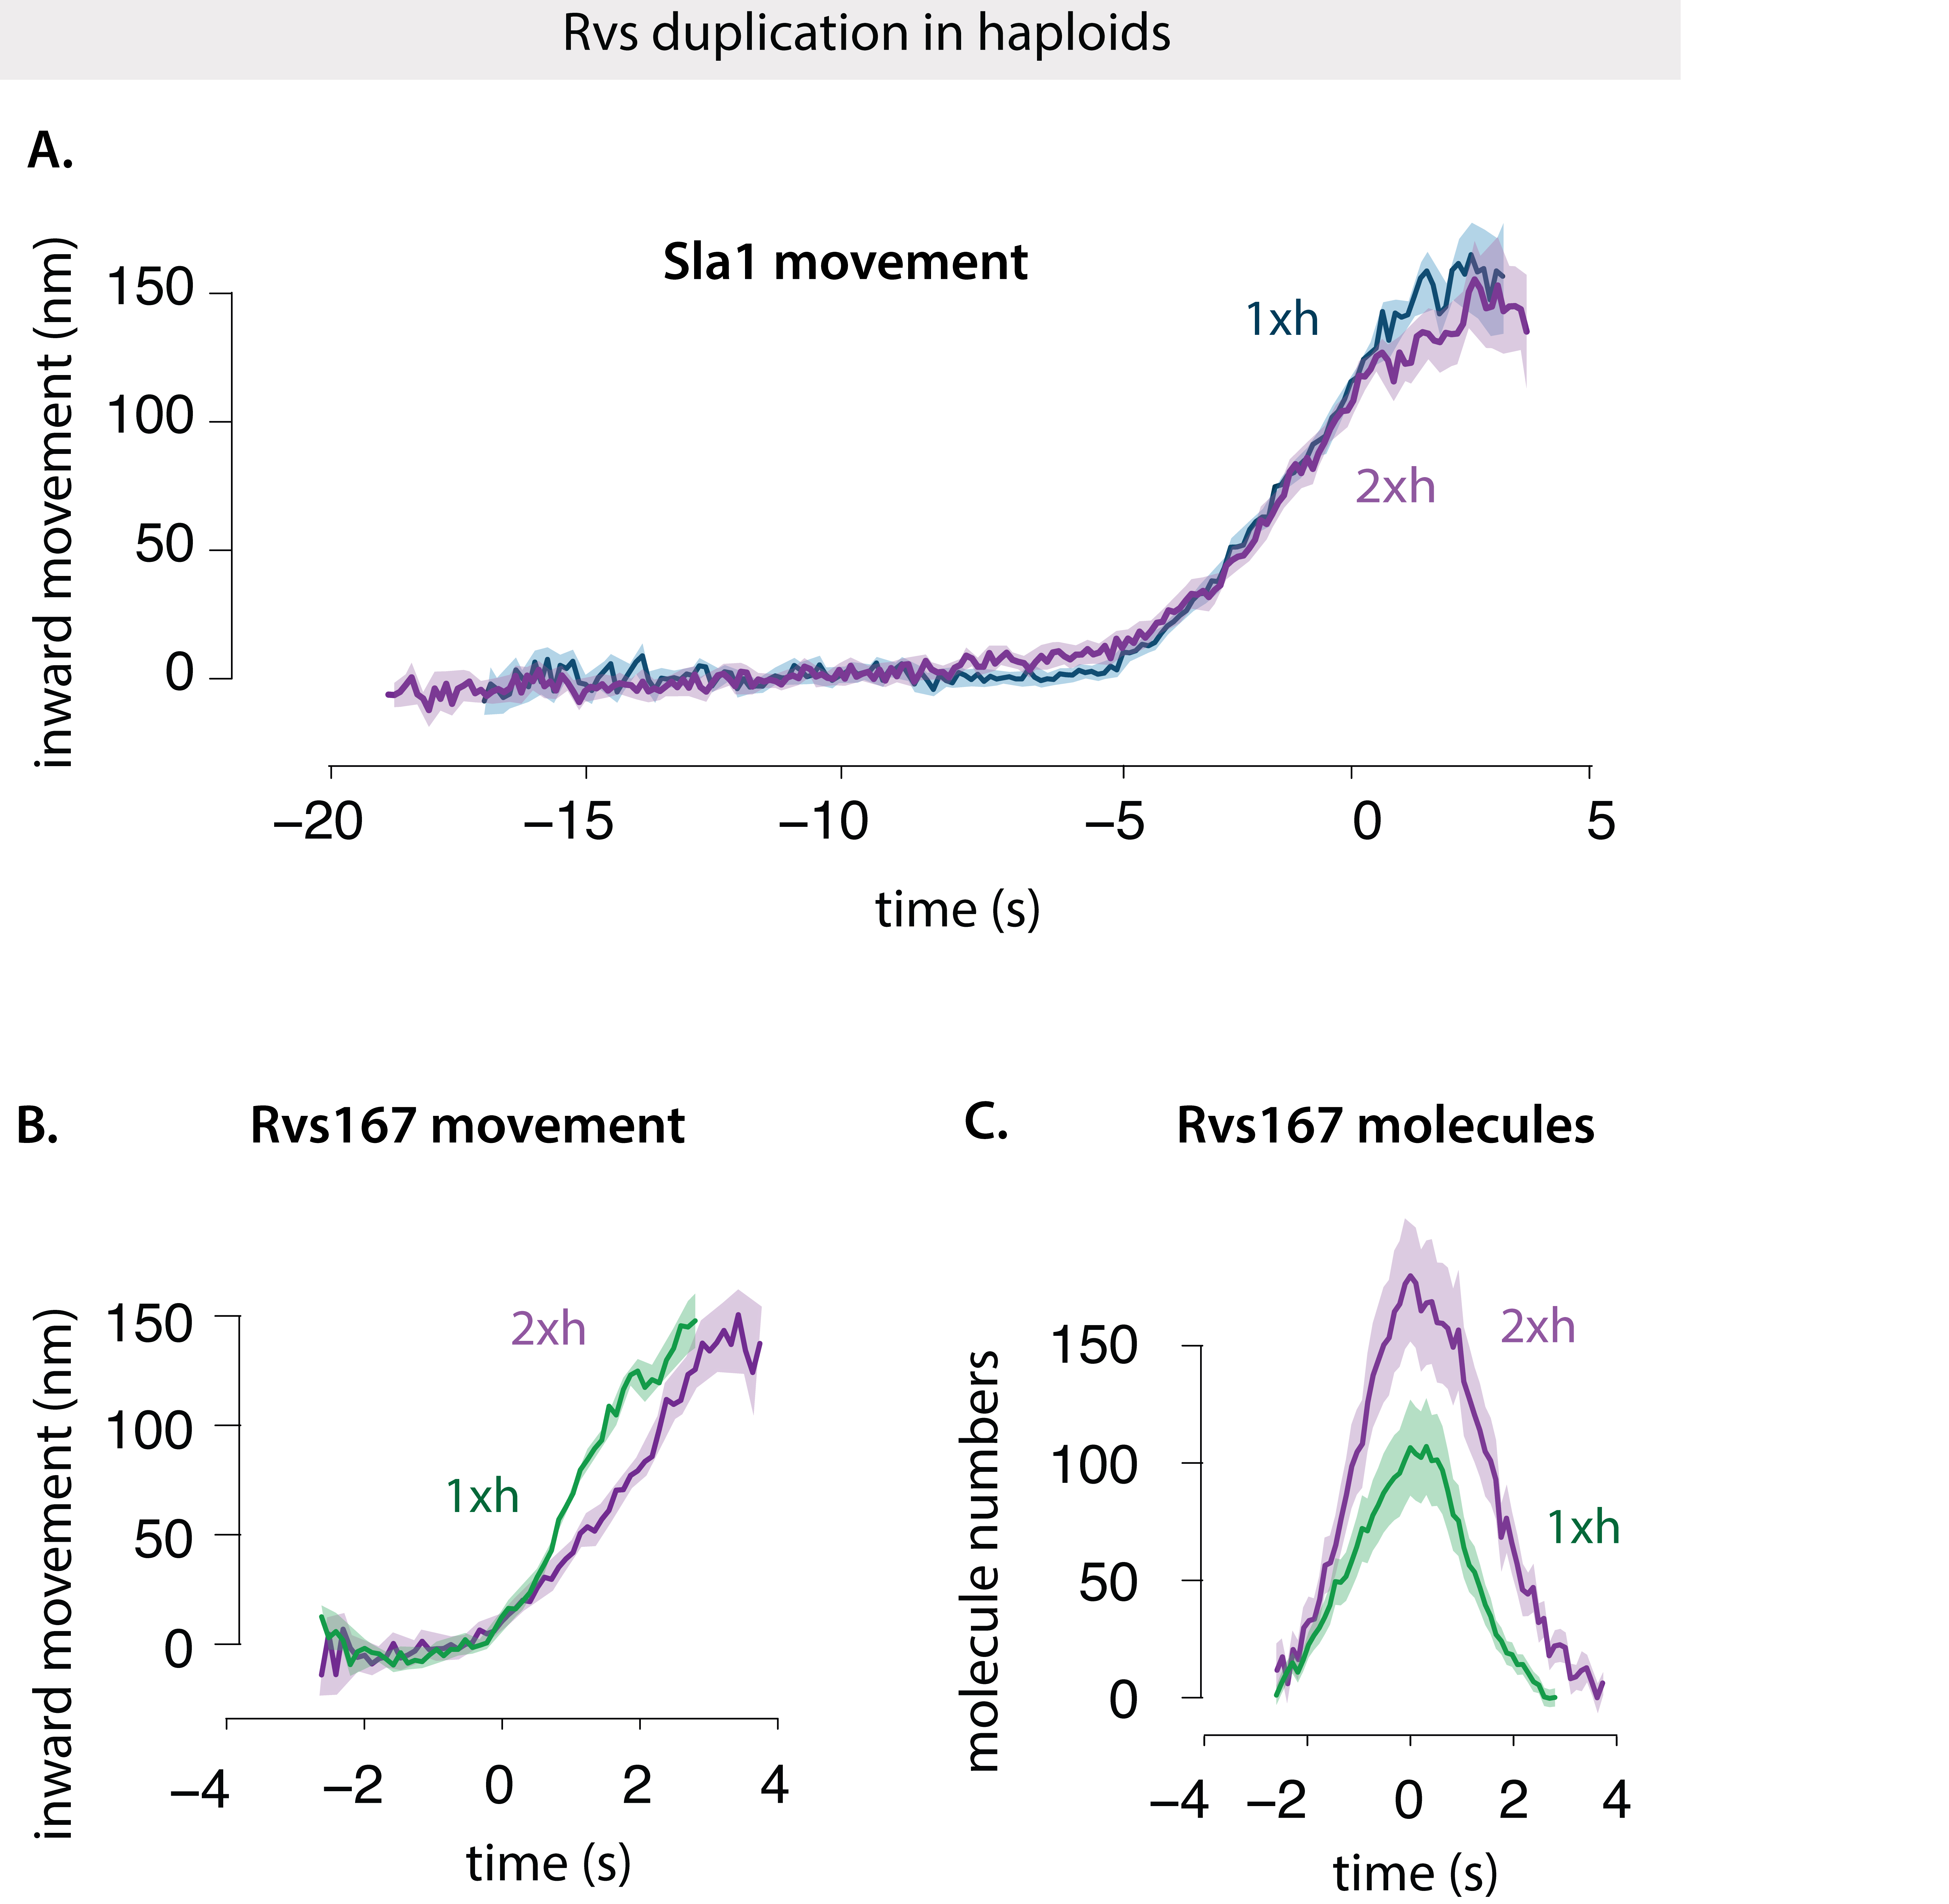
\includegraphics[width=15cm,height=15cm,keepaspectratio]{figures/results_final/rvs_haploid4}
	\vspace*{2mm}
	\caption[Overexpression of Rvs in haploid cells]
	{A. Movement Sla1 in haploid cells containing 1 (WT, 1xh) and 2 copies (2xh) of Rvs161, Rvs167 genes. Sla1 centroid in 1xh is aligned so that time=0 (s) corresponds to scission time. Centroid of 2xh Sla1-GFP is shifted to move inwards at the same time. 
		B. C Molecule numbers and movement of Rvs167 to sites in 1xh and 2xh cells. In B and C, 1xh is aligned to scission time. 2xh is shifted to move inwards at the same time as 1xh
		\label{fig_rvshaploid}}
	
\end{figure}
 %(Fig.\ref{fig_rvshaploid}B). 
 \underline{Sla1 and Rvs in Rvs duplicated haploids}
 
In Fig.\ref{fig_rvshaploid}A, Sla1 movement in WT (1xh) and duplicated (2xh) haploids are presented. WT Sla1 is aligned so that time= 0 (s) corresponds to scission time. Sla1 for 2xh is shifted so that it moves inward at the same time as WT. Both Sla1 centroids move inward at the same rate, and to the same distance of 140nm, suggesting that membrane progression is unchanged even if more Rvs is recruited. 

I measured the number of Rvs molecules recruited to endocytic sites in 1xh and 2xh strains. The maximum number of Rvs molecules recruited in the 2xh strain is 178 +/- 7.5, compared to 113.5 +/- 5.3 in WT (Fig.\ref{fig_rvshaploid}C): 1.6x more Rvs is recruited to endocytic sites in the gene duplicated strain. In Fig.\ref{fig_rvshaploid}C, fluorescent intensity of Rvs167 in 1xh and 2xh cells are shown. Both Rvs167 fluorescent intensity plots are aligned so that time=0 (s) corresponds to their respective maxima. Rvs accumulation takes the same amount of time in 1xh as in 2xh, so rate at which Rvs molecules is recruited to endocytic sites is 1.6x in Rvs duplicated cells (Fig.\ref{fig_rvshaploid}B). A much higher number of Rvs molecules can therefore be recruited to endocytic sites than is recruited in  WT cells, indicating that the recruitment of Rvs is influenced by the amount of available protein.

However, the dynamics of Rvs disassembly are quite different. Fig.\ref{fig_rvshaploid}B shows that disassembly is slowed by about 1.5 seconds in 2xh compared to 1xh cells. When comparing Rvs movement, (Fig.2.8C), instead of the sharp jump seen in WT, there is a delay in movement into the cytoplasm in 2xh cells. In WT cells, the sharp disassembly of Rvs indicates that all the protein is bound to the membrane: after scission, there is no tubular membrane, so all the Rvs is released at once. The delay in disassembly in the 2xh case then suggests that all the protein is not directly on the membrane. 
	\vspace{5mm}

		
%		\subparagraph{Sla1 and Rvs in gene duplicated diploids:}

		
\underline{Sla1 and Rvs movement is unchanged if more Rvs is recruited}
		\label{sub_rvsdiploids}
		
Compared to WT haploid strains expressing Rvs167-GFP, WT diploid strains appear to have more endocytic patches (Fig.2.10B). 
In diploid cells expressing 1 (1xd), 2 (2xd), and 4 (4xd) copies of the Rvs complex, Sla1 movement, Rvs dynamics, and recruitment of Rvs are compared. 
In Fig.\ref{fig_rvsdiploid1}A, Sla1 in the three cell types are shown. In all cases time=0 (s) corresponds to scission time. Sla1 movement is the same in 4xd and 2xd cells: they move at the same rate, and to the same lengths of about 140nm. In 1xd strain, Sla1 movement rate is the same till about 110nm, and is then slightly reduced. Sla1 movement in 1xd suggests that vesicle scission occurs at invagination lengths about 10nm shorter than that in 2xd and 4xd. 

\newpage
Rvs167 movement and fluorescent intensities are shown in Fig.\ref{fig_rvsdiploid1}B,C. 
Magnitude of inward movement of the Rvs is similar for the 4xd, 2xd and 1xd. In the 1x strain, however, the centroid disappears immediately after scission, suggesting that there is reduced Rvs at the base of the newly formed vesicle compared to the 2xd and 4xd.

	\vspace{5mm}
Recruitment dynamics of Rvs in all three are different: in the 4xd strain, Rvs is recruited at a rate of about 51 molecules/second, which is reduced to 27.5 molec./sec. for 2xd and 13.6 molec./sec. for the 1xd. Recruitment of Rvs is not directly proportionate to gene copy number: maximum number of Rvs recruited increases from 101 +/- 4.6 in the 2x Rvs strain to 143 +/- 5.5 in the 4x strain (see\ref{table1_numbers}). In the 1x Rvs strain, a maximum of 80 +/- 4.7 molecules of Rvs are recruited. In order to determine whether this is a reflection on protein availability or if something else limits recruitment of Rvs, I quantified the cytoplasmic intensities of Rvs167-GFP in the respective strains, and compared them to the WT intensity. The number of molecules recruited to endocytic sites scales with the amount of protein in the cytoplasm (see\ref{table2}).  



\vspace{2mm}
						\begin{figure}[H]
	\centering
\includegraphics[width=21cm,height=21cm,keepaspectratio]{figures/results_final/protein_friction7}
	\vspace*{2mm}
	\caption[Molecule numbers in diploid cells]
	{A. Maximum intensity projection of haploid and diploid cells expressing Rvs167-GFP. Scale bar =2um.      
		B. Maximum molecule number and standard error of mean of Rvs167-GFP and Abp1-mCherry in diploid strains. Only one allele of Abp1 is tagged with m-Cherry, so double the amount shown here is expected to be recruited. P-values from two-sided z test,  * = p$\leq$ 0.05, ** = p$\leq$ 0.01, *** = p$\leq$ 0.001. 
		\label{fig_rvsdiploid1}}
\end{figure}








%		\subparagraph{Abp1 amounts in gene duplicated diploids:}
\underline{Abp1 amounts in gene duplicated diploids:}
		
I measured the amount of Abp1 at endocytic sites in 4xd, 2xd, and 1xd diploid cells. Abp1 numbers provided in Fig.\ref{fig_rvsdiploid2}B are quantified in cells containing Rvs167-GFP and Abp1-mCherry. Abp1-mCherry signal was then scaled to Nuf2-mCherry, similar to quantification method in Picco et al. (2015). Fig2.10B shows that even though the number of Rvs molecules recruited varies depending on the number of Rvs gene copies, the same amount of Abp1 is recruited to endocytic sites in all three cases. In the Abp1 quantification in this case, only one allele of Abp1 is tagged with mCherry, the total amount of Abp1 is therefore likely to be double the numbers reported, although this assumes that labelled and unlabelled Abp1 are recruited at the same rate to endocytic sites. 

Rvs gene duplication data suggests that even if Rvs is recruited up to 1.6x faster than in WT cells, the maximum lengths of membrane invaginations do not change. The same amount of Abp1 is recruited irrespective of amount of Rvs, suggesting that membrane invagination is sensitive to amount of Abp1, and therefore actin, rather than Rvs. Sensitivity to the amount of actin suggests that scission timing is likely to be determined by the amount of force generated by the actin network. 


\vspace{3mm}
	\begin{figure}[H]
	\centering
	\hspace{-2cm}
	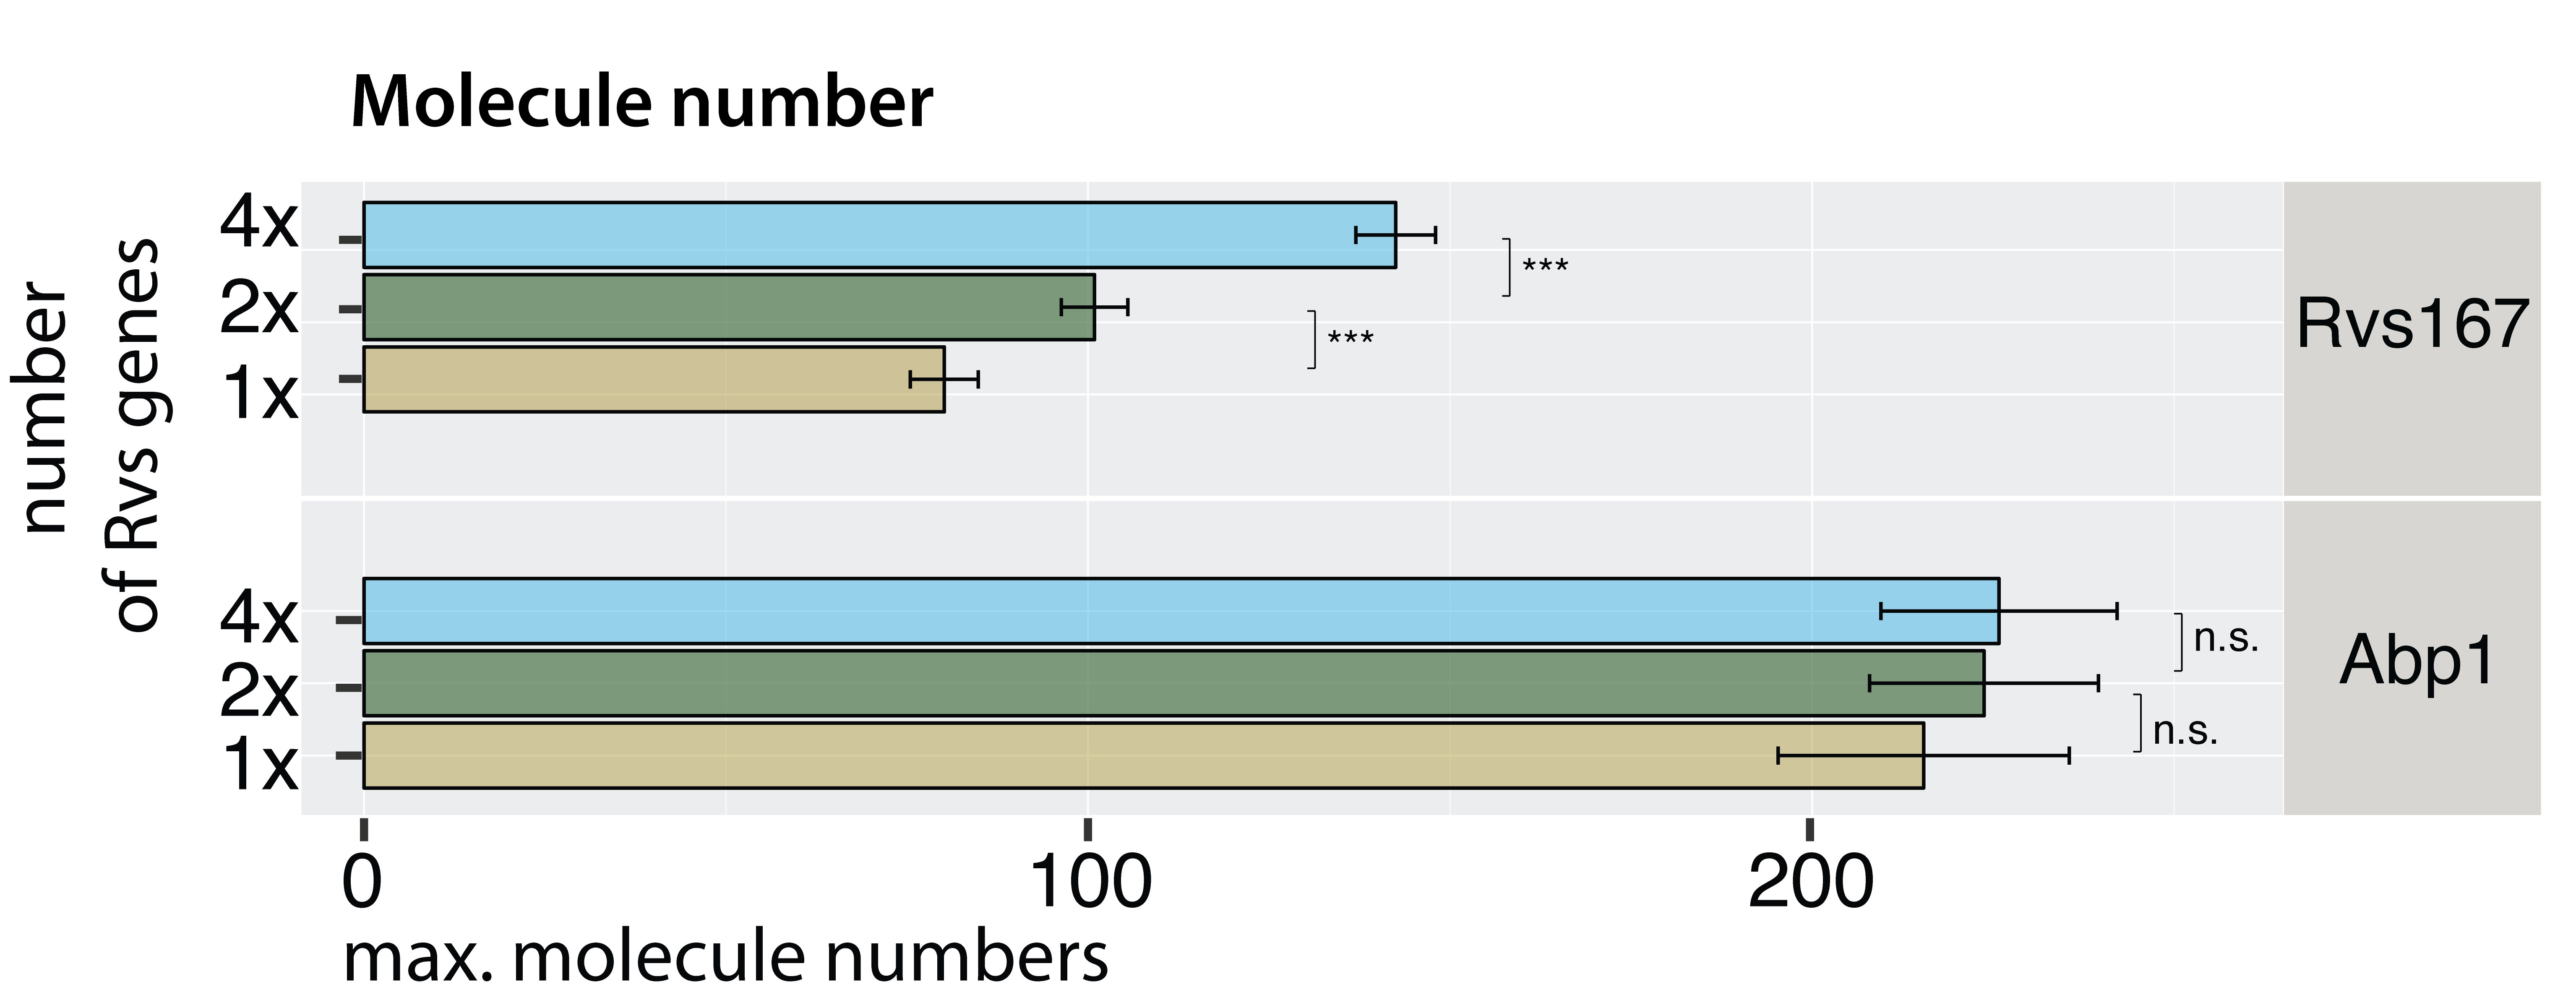
\includegraphics[width=15cm,height=15cm,keepaspectratio]{figures/results_final/protein_frictionB_4}
	\vspace*{2mm}
	\caption[Titration of Rvs molecule numbers in diploid cells]
	{A. Movement of Sla1 in diploid cells containing 1 (2xd), 2 (WT, 2xd) and 4 copies (4xd) of Rvs161, Rvs167 genes. Sla1 centroids for 2xd, 4xd are aligned so that Time=0 (s) corresponds to scission time. 1xd Sla1-GFP centroid is shifted to move inwards at the same time as the other two.
		B. Rvs167 movement in 1xd, 2xd and 4xd cells. All are aligned so that time=0 (s) corresponds to maximum molecules recruited.
		C.  Number of molecules of Rvs167-GFP in 1xd, 2xd, 4xd cells. Time=0 (s) corresponds to maximum molecules. 
		\label{fig_rvsdiploid2}}
\end{figure}




				
			




\newpage
%	\subparagraph{BAR domains as membrane scaffolds}
\subsection{Hypothesis: BAR domains scaffold the membrane, preventing scission}
				\mbox{}\\
As mentioned earlier in Section.\ref{scaffolding_rvs}, based on the capacity for BAR domains to oligomerize and tubulate liposomes, it has been proposed that membrane scaffolding is their \textit{in vivo} function. As membrane scaffolds, they would impose their own curvature on the underlying membrane and stabilize this shape. There are some requirements for a protein to act as a scaffold (Qualmann, Koch and Kessels, 2011):\\
	1. it must have a defined membrane interface\\
	2. it must have an intrinsic curvature\\
	3. it must be rigid in structure, and\\
	4. its membrane binding surface must be large enough to induce curvature\\

\vspace{-1mm}

BAR domains present a curved shape as the membrane interacting surface (Peter et al., 2004; Weissenhorn, 2005; Jennifer L Gallop, 2006), and have the capacity to oligomerize into large assemblies on tubes (Takei et al., 1999; Arkhipov, Yin and Schulten, 2009; Mim and Unger, 2012). It has also been shown that the central BAR region is rigid and is required for tubulation (Masuda et al., 2006). BAR domains therefore meet all of these requirements. 

	\vspace{5mm}
It has been shown that BAR domains can prevent membrane scission by scaffolding the membrane, allowing formation of stable tubular structures and preventing vesiculation of these structures (Boucrot et al., 2012). In simulations, adding BAR domains to an invaginating tube removes membrane shape instabilities. Actin forces, membrane rigidity and tension, and turgor pressure result in a wide invagination tip and shrinking tubular region that result in membrane shape instability and therefore scission. Adding curved BAR domains that have a preferred radius of curvature results in stabilization of the membrane shape and prevents scission (Dmitrieff and Nédélec, 2015).

	\subsubsection{Coat movement is influenced by recruitment of BAR domain }
As observed in the previous section \ref{sub_rvsdiploids}, Sla1 movement is decreased by reduced recruitment of Rvs, although adding excess protein (compared to the WT protein level) does not affect it. In BAR cells, Sla1 movement is reduced from WT to close to that of \textit{rvs167$\Delta$}. However, Rvs recruitment is also decreased in BAR cells compared to WT. Reduced coat movement therefore could result from loss of the SH3 domain, or from reduced BAR recruitment. To test this, I duplicated, as described before, the BAR domain alone in haploid yeast cells (2xBAR). I then compared Sla1 and Rvs in 2xBAR against BAR (1xBAR), WT Rvs (1xh), duplicated Rvs (2xh), and \textit{rvs167$\Delta$}

	\vspace{5mm}
 As shown in Fig.\ref{fig_scaffold}C,1x BAR is recruited at low copy numbers compared to WT. Maximum molecules recruited is 57 +/- 9.9, about 50\% that of WT. Recruitment of the BAR domain in 2x BAR is 90.58 +/- 9.6, 62\% of the WT levels. 
 
	\vspace{5mm}
In WT cells Sla1 moves inward at a rate of about 26 nm/s. While duplication of the full-length Rvs genes does not change the rate of inward movement of Sla1, total rate of inward movement is reduced to 13.3 nm/s in 1x BAR case. This rate increases to about 18 nm/s in the 2x BAR case. Adding BAR domain increases the rate of inward movement, as well as the distance Sla1 moves. Movement of Sla1 centroids in \textit{rvs167$\Delta$} cells is similar to 1x BAR case. Increasing the amount of BAR domain recruited to endocytic sites therefore shifts the movement of Sla1 from near \textit{rvs167$\Delta$} lengths to WT lengths (Fig.\ref{fig_scaffold}B,C).
	\vspace{5mm}
Shallow invaginations of the \textit{rvs167$\Delta$} can be rescued by adding Rvs molecules, whether BAR or full-length Rvs. In the 1xBAR case, since less Rvs is recruited, invaginations remain shallow, and the BAR domain has to be overexpressed to be recruited at near WT molecule numbers.
This shows that the coat movement is sensitive to the amount of Rvs, and needs only the BAR domain interaction.



		\begin{figure}[H]
	%	\centering
		\vspace*{-2 mm}
		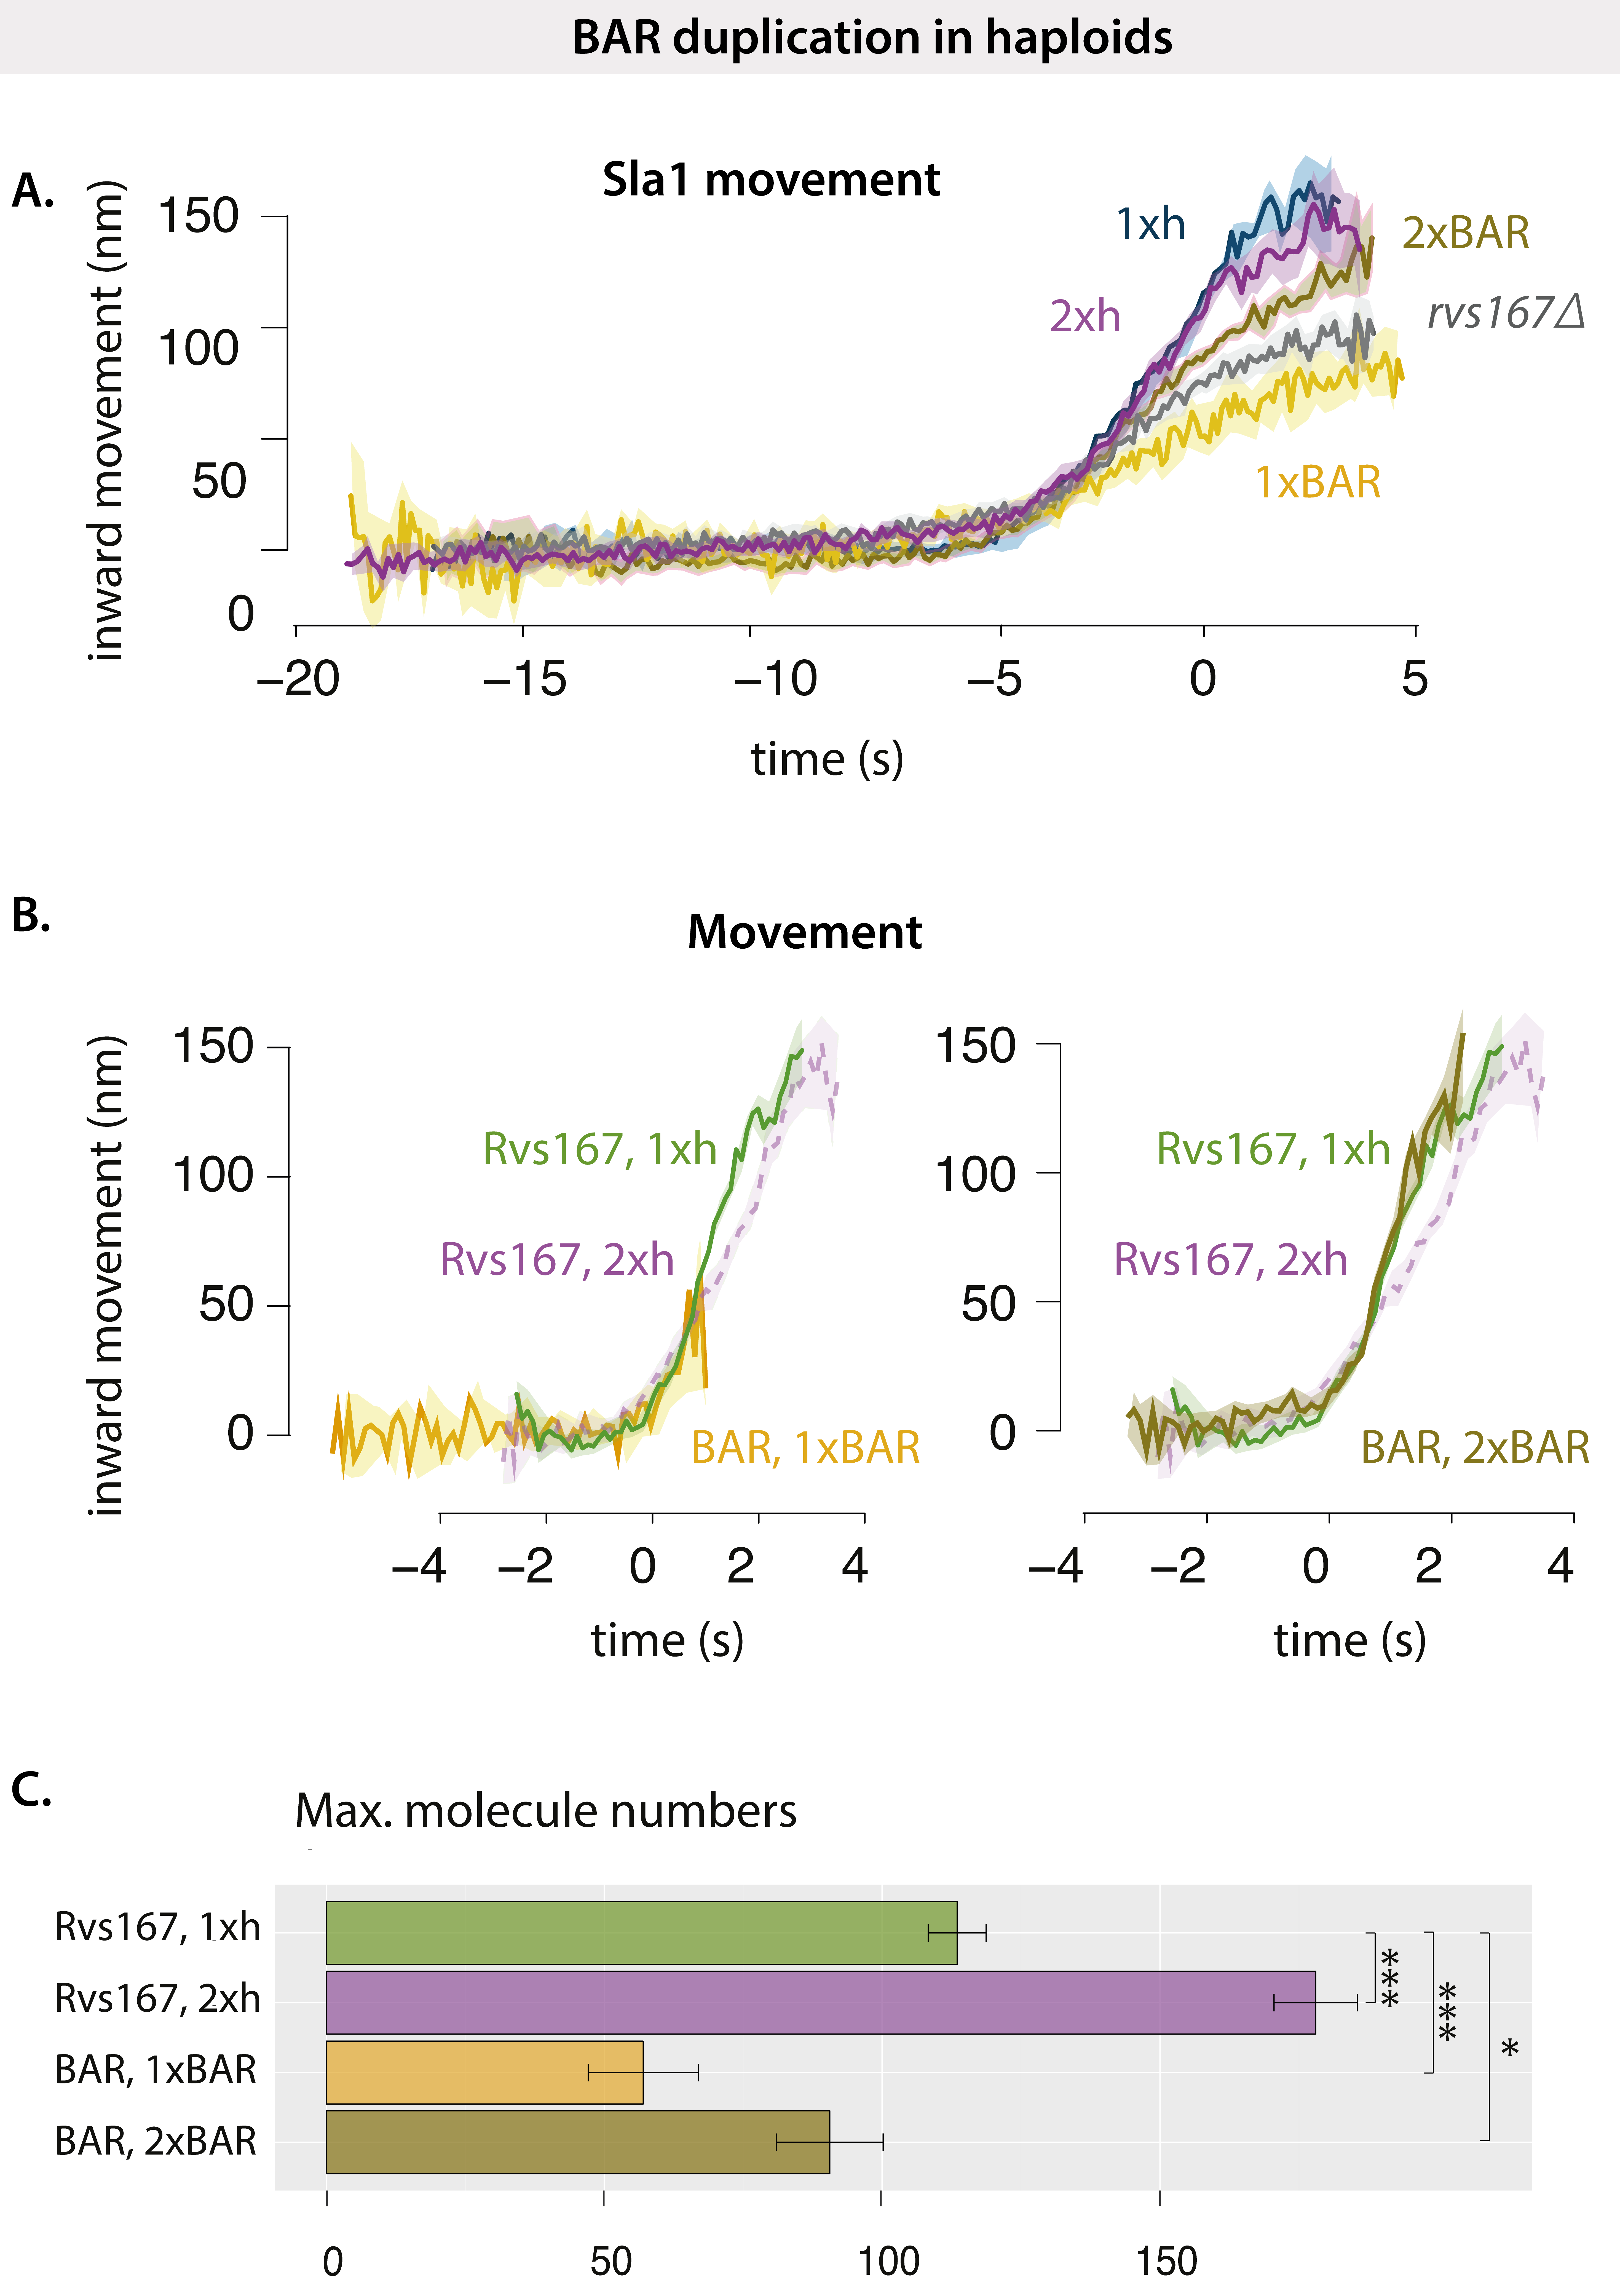
\includegraphics[width=21cm,height=21 cm,keepaspectratio]{figures/results_final/scaffolding_overlaid3}
		\caption [Overexpression of the Rvs BAR domain]
		{A: Movement of Sla1 in haploid cells consisting of 1 (WT, 1xh) and two copies (2xh) of Rvs genes, 1 (1xBAR) and 2 copies of BAR domain (2xBAR) and  \textit{rvs167$\Delta$} cells. Time=0 (s) for WT Sla1 is scission time. Other centroids shifted to move inwards at the same time as WT.
		B: Movement of Rvs167 in 1xh, 2xh, 1xBAR, 2XBAR cells. Time= 0 (s) for WT corresponds to scission time. Other centroids shifted to move inwards at the same time as WT.
		C: Maximum molecule number and standard error of mean of Rvs167-GFP at endocytic sites. P-values from two-sided z test, * = p$\leq$ 0.05, ** = p$\leq$ 0.01, *** = p$\leq$ 0.001. }
		\label{fig_scaffold}
		\end{figure}


\subsubsection{Hypothesis: Rvs ss a scaffold against turgor pressure} 
	
	\mbox{}\\
Intracellular pressure, membrane tension, and rigidity influence the shape of membrane invaginations. In yeast, turgor pressure has been estimated around 0.6 - 0.8 MPa pushes the plasma membrane against the cell wall. This pressure is opposed by the rigid cell wall, and the endocytic machinery must exert forces to bend and pull the plasma membrane away from the cell wall into the cytoplasm. Forces from actin polymerization are hence necessary to overcome this resistance to membrane invagination. In Dmitrieff and Nédélec, 2015, simulations show that membrane tension has a negligible influence on forces required to pull the membrane. Shape of the membrane is primarily influenced by membrane rigidity and turgor pressure. Membrane rigidity, which comes from the properties of the lipids and proteins embedded in it influences the shape of the top of the invagination that is pulled up. Actin forces are coupled to the top of the invagination, and turgor pressure pushes against the invagination, constricting the membrane neck.  

Turgor pressure can be controlled by osmoregulating agents like sorbitol. Sorbitol treatment causes cells to expel water and increase the internal concentration of osmolytes to match that of the environment. When the cell expels water, they shrink in size, resulting in a brief decrease of turgor pressure. Loss of turgor pressure is compensated by increased glycerol production in cells within 10 minutes of sorbitol treatment.


In fission yeast S.pombe, treatment with sorbitol shortens the time between arrival of the coat protein Sla1 and actin-binding protein App1, but does not affect the inward movement of the coat(Basu, Munteanu and Chang, 2014). Sorbitol rescues the invagination defect of partially blocking actin with low doses of LatA. At 0.2M sorbitol, 90\% of Sla1 patches in these cells move inward for 50nm instead of 300nm, but retract back to the plasma membrane. 


%\underline{Some WASP/Myosin mutations can be rescued by reducing turgor pressure. Deletion of myosin results in failure to invaginate, and this can be rescued up to 70\% when treated with 0.2 M Sorbitol. Loss of Fimbrin, which bundles actin filaments, and is also necessary for membrane invagination, can also be rescued by sorbitol.  These experiments show that some defects in the force generation system can be compensated by lowering turgor pressure.  Since sorbitol decreases the amount of time between App1 arrival and movement, reducing turgor pressure likely lowers the threshold force required to pull the membrane in the early stages of invagination. Consistent with this, simulations of Serge et al., show that the force requirement for membrane invagination is highest in the beginning of the invagination process.} 

An extension of the scaffold hypothesis for Rvs is that it protects the membrane tube against the high turgor pressure inside yeast cells. Reducing turgor pressure could then remove the requirement for Rvs scaffolding.

	\subsubsection{Requirement for Rvs is unchanged by membrane tension}

	In order to test if the role of the Rvs scaffold is to counter the membrane constricting effect of turgor pressure, I studied Sla1 and Rvs in WT and \textit{rvs167$\Delta$} cells treated with 0.2M sorbitol. At higher concentrations of sorbitol, cells shrivel and do not recover from turgor pressure loss(Basu, Munteanu and Chang, 2014).

	
		\begin{figure}[H]
		\centering
		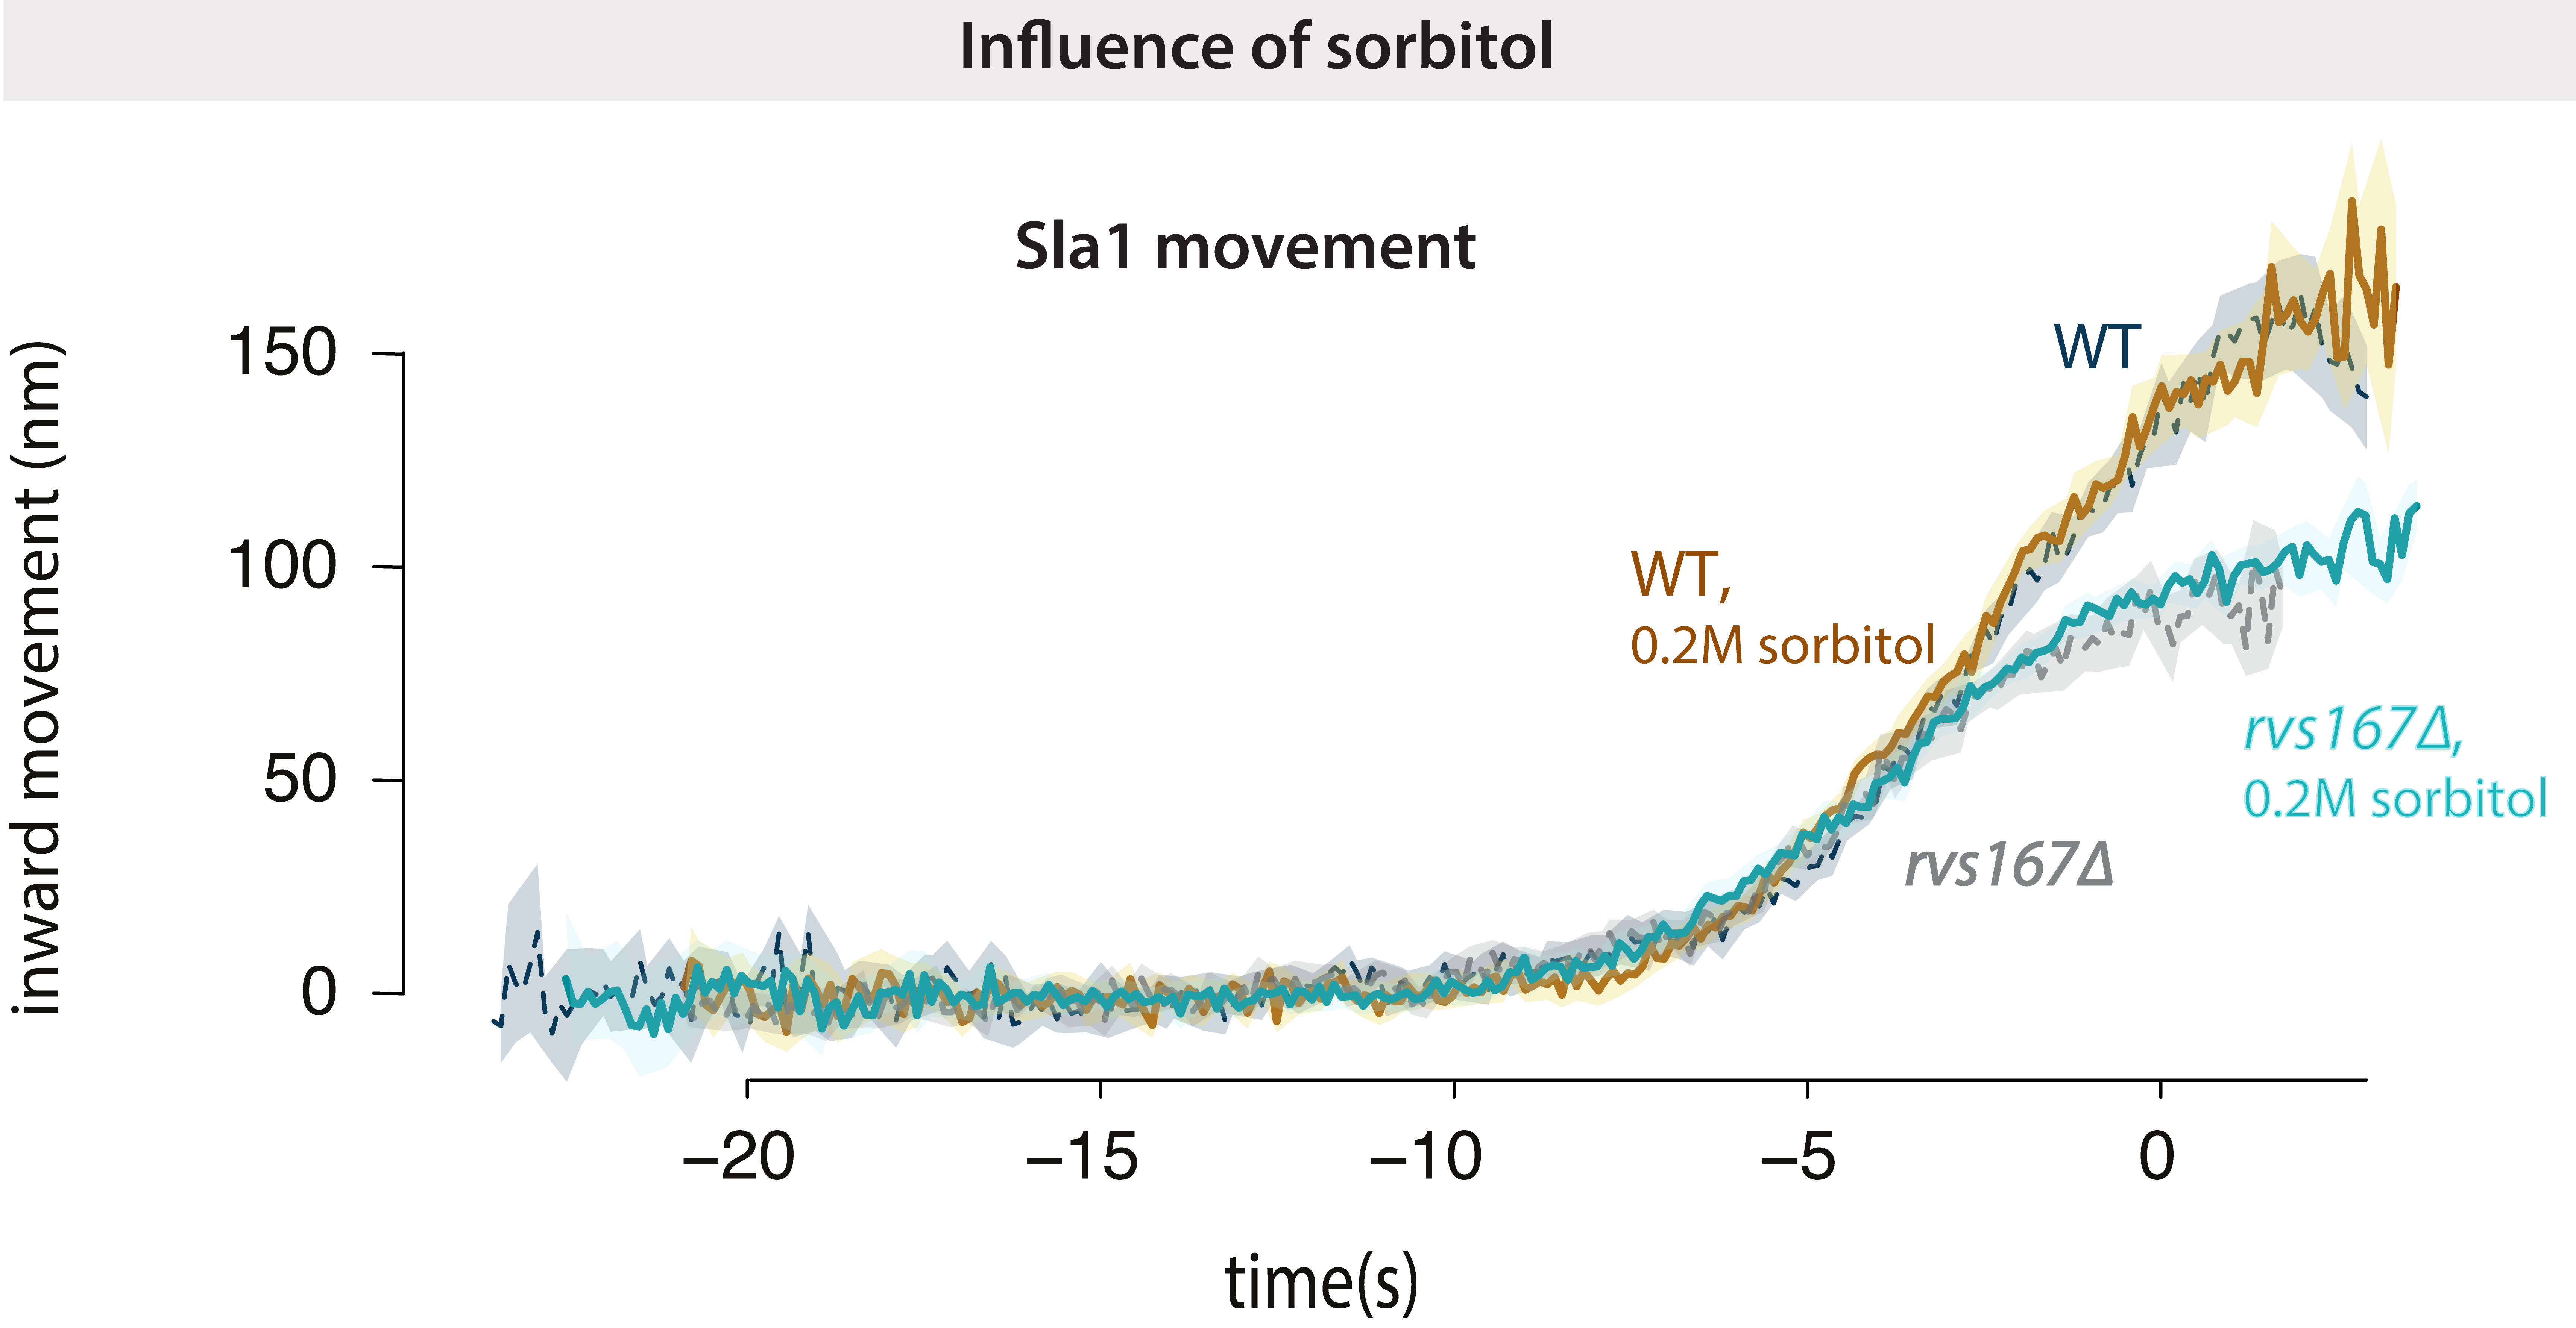
\includegraphics[width=15cm,height=17cm,keepaspectratio]{figures/results_final/sorbitol2}
		\caption[Effect of sorbitol on \textit{rvs167$\Delta$} cells]
		{Movement of Sla1-GFP in WT, WT cells treated with 0.2M sorbitol, \textit{rvs167$\Delta$} and \textit{rvs167$\Delta$} cells treated with 0.2M sorbitol. WT Sla1-GFP aligned to scission time, other centroids moved to move inwards at the same time as WT.
			\label{fig_sorbitol}}
		
	\end{figure}

In Fig.\ref{fig_sorbitol}, Sla1 movement in WT and \textit{rvs167$\Delta$} cells with and without sorbitol is shown. WT Sla1 is aligned so that time=0 (s) corresponds to scission time. The other three centroid movements are shifted so that they move inward at the same time as the WT. WT cells treated with sorbitol do not show any change in inward movement of Sla1. Both centroids move to the same lengths of 140nm at the same rate, consistent with S.pombe data from Basu et al. In \textit{rvs167$\Delta$} cells, Sla1 moves to about 80nm. In \textit{rvs167$\Delta$} cells treated with sorbitol, there is no difference in the movement. Both Sla1 centroids move at the same rate, and to the similar invagination lengths.

This result shows that the Rvs scaffold does not function to counter turgor pressure.  



\newpage
\begin{table}[H]
	\centering
	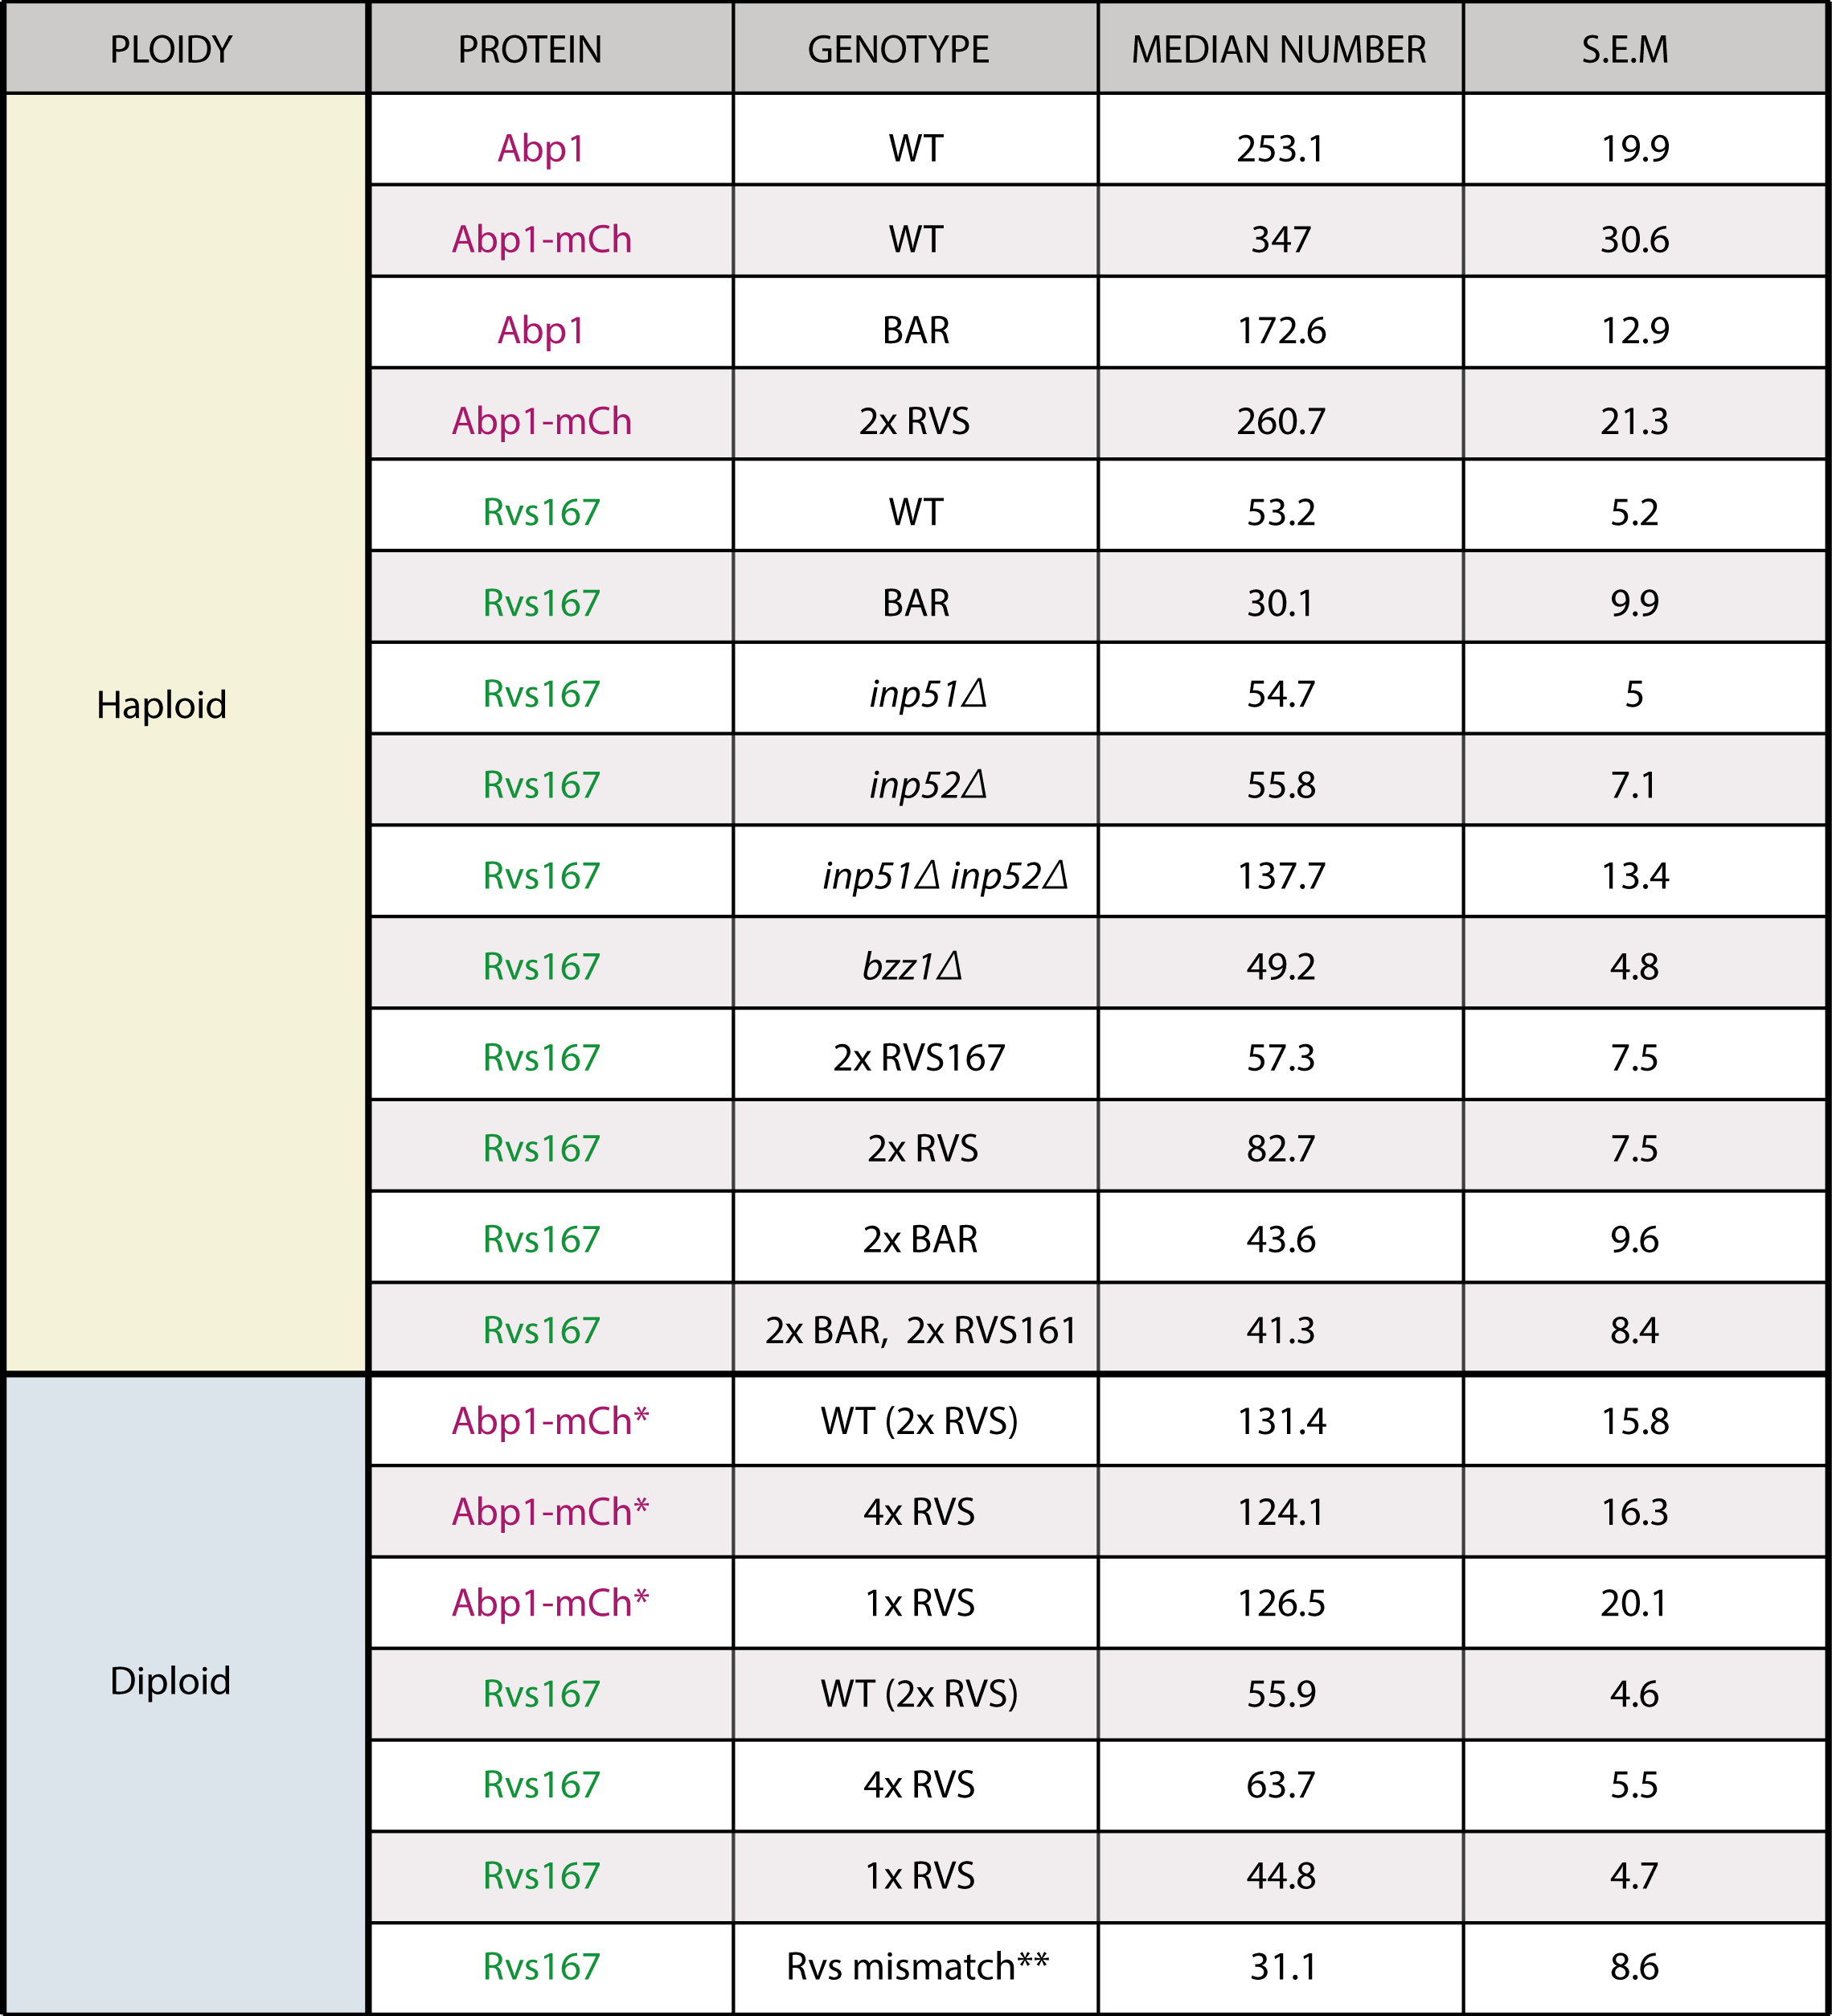
\includegraphics[width=15cm,height=30cm,keepaspectratio]{figures/results_final/table_numbers}
		\caption[Molecule number of Rvs167 and Abp1]
	{ Median molecule numbers of Rvs167 and Abp1 measured in different yeast strains. *= Number of molecules was quantified in cells containing one tagged allele of Abp1-mCherry. 
	\label{table1_numbers}}
	%	\caption[Median molecule numbers]
\end{table}

\newpage
\begin{table}[H]
	\centering
	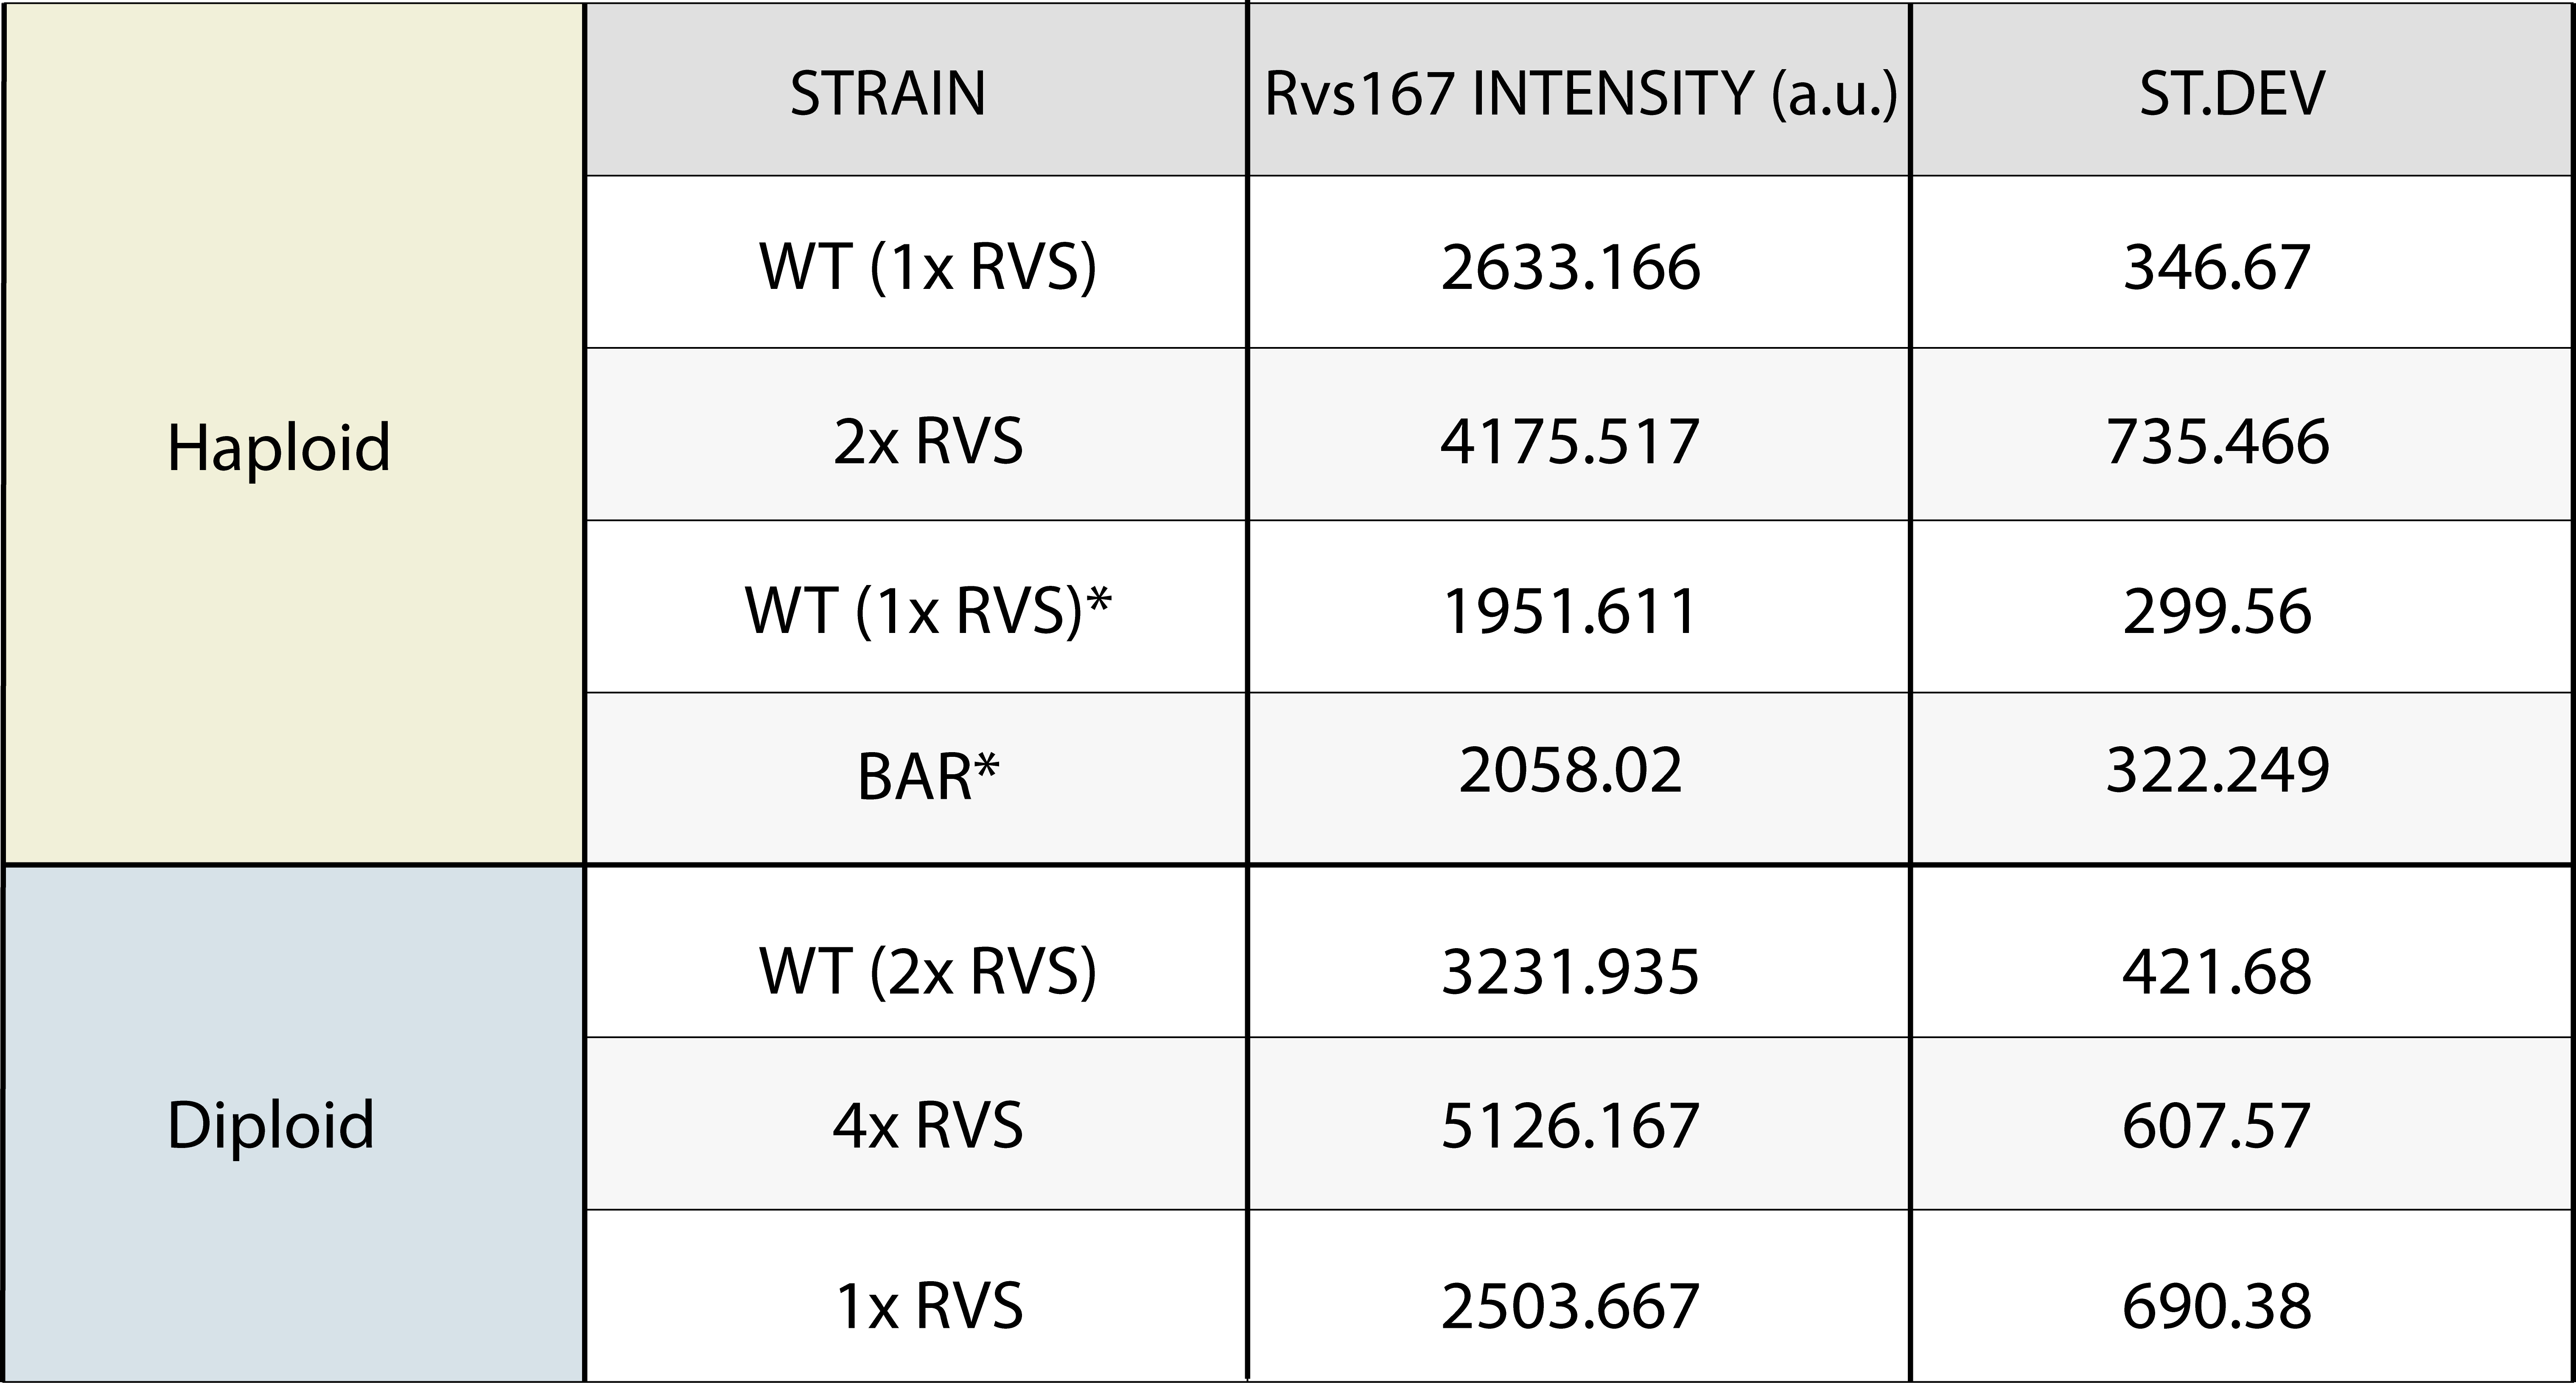
\includegraphics[width=13cm,height=25cm,keepaspectratio]{figures/results_final/table2}
	\caption[Cytoplasmic intensity quantification]
	{ Cytoplasmic intensity measured in different strains according to methods.
		\label{table2}}

\end{table}